\documentclass[a4paper, oneside, 11pt, openright]{book}


\usepackage[a-1b]{pdfx}
\usepackage{cite}
\usepackage{geometry,url,graphicx, hyperref,subfig,enumitem, amsmath,float}
\usepackage{amsmath, amssymb, amsthm, mathtools, color, setspace}
\usepackage{fancyhdr, braket, etoolbox,booktabs,multirow}
\usepackage{xfrac, lmodern, ifsym, bm, multicol, booktabs, pdflscape} % xfrac gives font errors, add lmodern to remove them. Check whether this re, mains a problem!
%\usepackage{hyperref}
%\usepackage[utf8]{inputenc}
%\usepackage{colorprofiles}
\usepackage[T1]{fontenc}

\usepackage{tikz-cd}

\usepackage{stackengine}
\def\tanslant{.25}
\newcommand\hatsrm[2][2]{\ensurestackMath{%
		\ifnum#1>1%
		\stackengine{-4pt}{\hatsrm[\numexpr#1-1\relax]{#2}}{%
			\scriptstyle\char'136}{O}{c}{F}{T}{S}%
		\else%
		\stackengine{-3pt}{#2}{\scriptstyle\char'136}{O}{c}{F}{T}{S}%
		\fi%
}}
\newcommand\hatsit[2][2]{\ensurestackMath{%
		\sbox0{$#2$}%
		\ifnum#1>1%
		\stackengine{-4pt}{\hatsit[\numexpr#1-1\relax]{#2}}{%
			\kern\tanslant\ht0\scriptstyle\char'136}{O}{c}{F}{T}{S}%
		\else%
		\stackengine{-3pt}{#2}{\kern\tanslant\ht0\scriptstyle\char'136}%
		{O}{c}{F}{T}{S}%
		\fi%
}}



\begin{document}
	\begin{titlepage}
		%%%% LOGO %%%%
		\begin{figure}
			\includegraphics[width=\linewidth]{thesis_images/logo.jpg}
		\end{figure}
		\begin{center}
			\textsc{\large Corso di laurea in Fisica}\\[0.2cm]
			\textsc{\normalsize Tesi di laurea magistrale}\\[2cm]
			%\rule{\linewidth}{0.3mm} \\[1.2cm]
			
			% TITLE
			\begin{doublespace}
				\textbf{\LARGE Search for new resonances in the 105 to 200 GeV diphoton invariant mass range using 140 fb$^{-1}$ of $pp$ collisions collected at $\sqrt{s}$=13 TeV with the ATLAS detector}
				\\[2cm]
			\end{doublespace}
			
			% AUTHOR
			\begin{minipage}{0.4\textwidth}
				\begin{flushleft}
					\emph{Autore:} \\[0mm]
					\textbf{Pietro Daniele} \\[4mm]
					\emph{Matricola:}\\
					982369 \\[4mm]
					\emph{Codice P.A.C.S.:}\\[0mm]
					12.60.Fr
				\end{flushleft}
			\end{minipage}
			%
			\begin{minipage}{0.4\textwidth}
				\begin{flushright} 
					\emph{Relatore:} \\
					\textbf{Prof. Leonardo Carlo Carminati} \\[1.2em]
					\emph{Corelatori:} \\
					\textbf{Dott. Ruggero Turra} \\
					\textbf{Dott.ssa Elena Mazzeo} \\[1.2em]
				\end{flushright}
			\end{minipage}\\[2cm]
			\vfill
			Anno accademico 2021-2022
		\end{center}
		
		
	\end{titlepage}
	
	\clearpage\null\thispagestyle{empty}\newpage
	
	\tableofcontents
	
	\chapter*{Introduction}\addcontentsline{toc}{chapter}{Introduction}
	
		In 2012, the ATLAS and CMS Collaborations discovered a new boson \cite{higgs_atlas},\cite{higgs_cms}, with mass $\sim$125 GeV, that was consistent with the Higgs boson predicted by the Standard Model of particle physics (SM). Its discovery confirmed the Higgs mechanism for the electroweak symmetry breaking.
		
		While the measurements of the production and decay rates of the 125-GeV Higgs boson (Higgs$_{125}$) are presently consistent with the predictions for the SM Higgs boson, there is no requirement for the Higgs sector to be minimal. Extended Higgs sectors, involving multiple scalar fields, can address some of the shortcomings of the SM. For example, the SM provides no dark matter candidate and no explanation for the matter-antimatter asymmetry in the universe. Hence, these phenomena can only be explained by new physics beyond the Standard Model (BSM). On a more theoretical level, %the vast discrepancy between aspects of the weak nuclear force and gravity, 
		the difference in scales between the mass of the Higgs boson and the Planck mass, called hierarchy problem, has puzzled physicists for a long time and continues to do so. Moreover, the SM does not explain its own flavor structure, nor does it yield coupling unification at high energy scales\cite{ext_higgs}. Therefore the Higgs field that forms in the SM a complex doublet under the weak isospin SU(2) symmetry group could be extended. Larger scalar sectors that include a boson consistent with the Higgs$_{125}$ observation typically incorporate this complex doublet and add additional structure, predicting new bosons. The extended Higgs sector can be embedded in a larger theoretical scenario, such as a two-Higgs-doublet model (2HDM)\cite{Branco_2012}, or supersymmetry (SUSY) \cite{dine_2016}.%, or it can be extended to include dark matter candidates.
		
		%The Higgs field in the SM forms a complex doublet under the weak isospin SU(2) symmetry group. Larger scalar sectors that include a boson consistent with the Higgs$_{125}$ observation typically incorporate this complex doublet and add additional structure. There can be additional real or complex singlets, doublets, triplets, and forth, or a combination of them. One of such completion could be a two-Higgs-doublet model (2HDM)\cite{Branco_2012}, that gives rise to two neutral and two charged additional Higgs bosons. The extended Higgs sector also can be embedded in a larger theoretical scenario, such as supersymmetry (SUSY) \cite{dine_2016}, or it can be extended to include dark matter candidates. The theoretical approaches can be divided into two categories, bottom-up and top-down approaches. In bottom-up approaches, pure extended scalar sectors are explored in a general fashion and can be considered as low-energy representations of an unknown larger theory at higher scales. In top-down approaches, the extended scalar sector is an intrinsic part of a concrete larger theoretical scenario. The most well-studied full model is the minimal supersymmetric Standard Model (MSSM) \cite{Djouadi_2008}. The MSSM addresses several shortcomings of the SM: it provides a dark matter candidate, allows for the unification of the gauge couplings, and mitigates the hierarchy problem. The MSSM requires a 2HDM-like Higgs sector. More complex models, such as a 2HDM with an additional singlet or a model with an additional triplet, typically reproduce at least part of the phenomenology of singlets and 2HDMs but can add interesting new phenomenology \cite{Dawson_2019}\cite{PhysRevD.98.030001}.
		
		The main phenomenological consequence of extended scalars sector is that they lead to additional states, which can manifest as additional neutral and charged scalars (commonly referred to as additional Higgs bosons) \cite{ext_higgs}\cite{Englert_2014}. These states can be produced directly at high-energy colliders and can in turn decay into various final states based on their mass and couplings. One of these decay channels is the di-photon final state: a search for spin-0 new resonances, in addition to Higgs$_{125}$, can be performed using the di-photon channel. %While the $\gamma\gamma$ branching fraction is subdominant, the searches in this final state profit from an excellent mass resolution and manageable backgrounds. 
		
		Searching for additional Higgs boson from $pp$ collisions in the two photons final states provides a considerable advantage, with respect to other decay channels. Such a search would| profit from the exceptional trigger and reconstruction efficiency for photons with the ATLAS detector and from the excellent invariant mass resolution of the di-photon system (1-2 GeV). Hence, an additional Higgs boson would appear, in the $m_{\gamma\gamma}$ spectrum, as a new peak, centred around the mass $m_X$ of the new particle. Therefore, in this thesis, a search for new spin-0 resonances, in addition to the 125-GeV SM Higgs boson, will be performed in the $\gamma\gamma$ channel in the [105,200] GeV invariant mass range. Searches have been carried out for $m_X$ near 125 GeV in the context of the SM Higgs boson analysis \cite{Lanyov_2014} as well as for higher \cite{2021136651}\cite{2017105} and lower masses (65 < $m_X$ < 110 GeV) \cite{ATLAS-CONF-2018-025}. None of these analyses showed a significant signal excess above the background-only expectations. A search for resonances in the $\gamma\gamma$ final state, in the considered mass range, suffers from a background from di-photon production from QCD processes, whose rate is three order of magnitude greater than the SM production. Therefore, employing a di-photon selection and an events categorisation, that enhances the signal over background rate, is crucial for improving the sensitivity of this analysis.
		
		After applying selection requirements obtaining pairs of high-$p_T$ and isolated photons, these events will be classified into mutually exclusive categories designed to both enhance the analysis sensitivity to new resonances and minimise the model dependence. Different categorisations are tested and compared with each other:  \texttt{Inclusive}, in which there is only one category which contains all selected events, \texttt{catConvEta}, which classifies the events in 6 different categories based on $\gamma$ conversion status and $\eta$ position, and \texttt{catConv}, which separates the events using $\gamma$ conversion status in two different categories. After the categorisation, the signal and background processes are modelled in the $m_{\gamma\gamma}$ spectrum. The signal in each category is defined as a function of the mass of the resonance and its model is created using simulated MC samples of SM (spin0) Higgs bosons decaying into two photons. The non-resonant background in each category is described by a smoothly falling function whose normalization and shape parameters will be determined from data, using a function form modelled using MC samples. In order to investigate the presence of new spin-0 resonances, the SM Higgs$_{125}$ is also included as background and modelled with a fixed resonant function. Once the categorisation are applied and the models are created, the results are extracted with a combined maximum likelihood fit in all the categories. The sensitivity of each tested categorisation is quantified by computing the compatibility of the representative MC data with the background-only hypothesis (i.e. calculating the $p$-values). Additionally, upper limits on the production cross-section, under the assumption of no signal, are set in order to estimate the analysis sensitivity. Looking at limits on the signal cross for each models built with different categorisation, the best working point is selected. The best categorisation is obtained from the trade-off between performances and model independence.
		
		This thesis is organized as follows. Chapter \ref{chapter:1} provides a description of the Large Hadron Collider and the ATLAS experiment. The photon reconstruction algorithm is described in Chapter \ref{chapter:2}. Chapter \ref{chapter:3} provides a general overview of statistical techniques used in particle physics. Chapter \ref{chapter:4} presents the MC samples, the signal and backgrounds models and the categorisation used in this analysis and its results. The conclusions are summarized in the final Chapter \ref{chapter:5}.
	
	\chapter{LHC and ATLAS Detector}\label{chapter:1}
		\section{LHC}
			The Large Hadron Collider (LHC) \cite{LHC_DESIGN_2008} is a two-ring, superconducting proton and heavy ions accelerator and collider installed in the 27 km long LEP \cite{LEP_DESIGN_2001} tunnel. The LHC was designed to provide $pp$ collisions at centre of mass collision energies of up to 14 TeV. 
			
			Inside the accelerator, two high-energy particle beams travel close to the speed of light before they are made to collide. To collide two beams of equally charged particles requires opposite magnet dipole fields in both beams. The LHC is therefore designed as a proton-proton collider with separate magnet fields and vacuum chambers in the main arcs and with common sections only at the insertion regions where the experimental detectors are located. 
		
			\subsection{LHC layout}
				The basic layout of the LHC \cite{LHC_DESIGN_2004} follows the LEP tunnel geometry (Figure \ref{fig:LHC_layout}). The LHC has eight arcs and eight straight sections. Each straight section ("insertion") is approximately 528 m long and can be used for beam collisions or utilities purposes (injection, beam dumping or cleaning). The two high luminosity experimental insertions are located at diametrically opposite straight sections: the {ATLAS} experiment is located at point 1 and the CMS experiment at point 5. Two more experimental insertions are located at point 2 and point 8 which also contain the injection systems for Beam 1 and Beam 2, respectively. The remaining four straight sections do not have beam crossings. Insertion 3 and 7 each contain two collimation systems. Insertion 4 contains two RF systems: one independent system for each LHC beam. The straight section at point 6 contains the beam dump insertion where the two beams are vertically extracted from the machine using a combination of horizontally deflecting fast-pulsed ("kicker") magnets and vertically-deflecting double steel septum magnets. Each beam features an independent abort system.
				
				\begin{figure}[H]
					\centering
					\includegraphics[width=0.5\textwidth]{thesis_images/lhc.jpg}
					\caption{LHC structure.}
					\label{fig:LHC_layout}
				\end{figure}
				
				\begin{figure}[H]
					\centering
					\subfloat[][\emph{LHC dipole}]{\includegraphics[width=.57\textwidth]{thesis_images/m_dipole.jpeg}} \quad
					\subfloat[][\emph{LHC quadpole}]{\includegraphics[width=.4\textwidth]{thesis_images/m_quad.png}} 
					\caption{LHC's superconducting magnets.}
					\label{fig:magnets}
				\end{figure}
				
				The LHC beams are controlled by superconducting magnets, which have a working temperature of 1.9 K. There are two kinds of superconducting magnets (Figure \ref{fig:magnets}):
				\begin{itemize}
					\item the superconducting dipole magnets, which thanks to a 8.33 T magnetic field drive protons along the ring (circular orbit);
					\item superconducting quadrupole magnets, which keep the beams focused.
				\end{itemize} 
					
			\subsection{CERN accelerator complex}
				The aim of the CERN accelerator complex (Figure \ref{fig:CERN_complex}) is to accelerate the particles beams, which could be inserted into the LHC ring. The accelerator complex a succession of machines that accelerate particles to increasingly higher energies. Each machine boosts the energy of a beam of particles before injecting it into the next machine in the sequence. In the Large Hadron Collider (LHC), which is the last element in this chain, particle beams are accelerated up to the record energy of 6.5 TeV per beam. In April 2022, after over three years of upgrade and maintenance work, the LHC started the Run3 phase, running at the record energy of 13.6 TeV, providing greater precision and discovery potential. Therefore thanks to the increased collision rates, higher collision energy, upgraded data readout and selection systems, new detector systems and computing infrastructure, a new physics season, which will further expand the already very diverse LHC physics programme, has started.
				
				Linear accelerator 4 (Linac4) has become the source of proton beams for the CERN accelerator complex in 2020. It accelerates negative hydrogen ions to 160 MeV to prepare them to enter the Proton Synchrotron Booster (PSB). The ions are stripped of their two electrons during injection from Linac4 into the PSB, leaving only protons. These are accelerated to 2 GeV for injection into the Proton Synchrotron (PS), which pushes the beam up to 26 GeV. Protons are then sent to the Super Proton Synchrotron (SPS), where they are accelerated up to 450 GeV. The protons are finally transferred to the two beam pipes of the LHC. The beam in one pipe circulates clockwise while the beam in the other pipe circulates anticlockwise. It takes 4 minutes and 20 seconds to fill each LHC ring, and 20 minutes for the protons to reach their maximum energy of 6.5 TeV. Beams circulate for many hours inside the LHC beam pipes under normal operating conditions. The two beams are brought into collision inside four detectors (ALICE, ATLAS, CMS and LHCb) where the total energy at the collision point is equal to 13 TeV. In addition to accelerating protons, the accelerator complex can also accelerate lead ions.
				
				\begin{figure}
					\centering
					\includegraphics[width=0.9\textwidth]{thesis_images/CERN_complex.png}
					\caption{CERN accelerator complex.}
					\label{fig:CERN_complex}
				\end{figure}
			
			\subsection{Proton-proton collisions}
				The number of events $R_{i}$ per second of a process characterized by a cross section $\sigma_{i}$ produced by the LHC collisions is given by:
				$$
				R_{i} = L\sigma_{i}
				$$
				where $L$ is the instantaneous machine luminosity. $L$ depends only on the beam parameters and can be written for a Gaussian beam distribution as: 
				$$
				L = \frac{N_b^2n_bf_{rev}\gamma_r}{4\pi\epsilon_n\beta^*}F
				$$
				where $N_b$ is the number of particles per bunch, $n_b$ the number of bunches per beam, $f_{rev}$ the revolution frequency, $\gamma_r$ the relativistic gamma factor, $\epsilon_n$ the normalized transverse beam emittance, $\beta^*$ the beta function at the collision point and $F$ the geometric luminosity reduction factor due to the crossing angle at the IP. 
				
				\begin{figure}
					\centering
					\includegraphics[width=0.5\textheight]{thesis_images/peakLumiByFill.pdf}
					\caption{The peak instantaneous luminosity delivered to ATLAS during stable beams for pp collisions at 13 TeV centre-of-mass energy per fill 2018.}
					\label{fig:insta lum}
				\end{figure}
				
				For the nominal value of the luminosity $10^{34}$cm$^{-2}$s$^{-1}$ the total inelastic proton-proton cross-section is about 80 mb at $\sqrt{s} = 14$ TeV. Therefore, the event rate $R$, defined as the number of events produced per second by the pp interactions, is expected to be:
				$$
				R = \sigma L = 80 mb\times10^{34}cm^{-2}s^{-1} \simeq 10^{9}s^{-1}.
				$$ 
				The number of events for each process is related to the integrated luminosity, shown in Figure \ref{fig:Integreted Luminosity}. For the LHC runs, the instantaneous luminosity reached the record value of $\sim 2 \cdot 10^{34}$ cm$^{-2}$s$^{-1}$ (Figure \ref{fig:insta lum}), a factor of two larger then the design value.
				
				\begin{figure}
					\centering
					\includegraphics[width=0.5\textheight]{thesis_images/intlumivsyear.pdf}
					\caption{Luminosity measured in inverse femtobarn versus time for 2011-2018 (p-p data only).}
					\label{fig:Integreted Luminosity}
				\end{figure}
				
				In a hadron collider, there are typically two types of $pp$ collisions:
				\begin{itemize}
					\item \textbf{Soft collisions}: 
					they are the most frequent and they are large-distance collisions between the two incoming protons. They are called "soft" because the momentum transfer of the interaction is small. Due to this feature, particle scattering at large angle is suppressed and so, after collisions, particles have a large longitudinal momentum, but small transverse momentum ($<p_T>\simeq500$ MeV) relative to the beam line. The final states
					arising from such interactions are called minimum bias events.
					\item \textbf{Hard collisions}:
					monochromatic proton beams can be seen as beams of partons (quarks and gluons) with a wide band
					of energy. Occasionally, head-on collisions occur between two partons of the incoming protons. These are interactions at small distances, and therefore are characterised by large
					momentum transfers ("hard scattering"). In this case, particles in the final state can be produced at large angles with respect to the beam line (high $p_T$) and massive particles can be created.
					These are the interesting physics events at a collider but they are, however, rare compared to the soft interactions.
					
					In the hard-scattering interactions of quarks and gluons at a hadron collider, the effective centre-of-
					mass energy of the interaction ($\sqrt{\hat{s}}$) is smaller than the centre-of-mass energy of the machine ($\sqrt{s}$) and is given by: 
					$$ 
					\sqrt{\hat{s}} = \sqrt{x_ax_bs}
					$$
					where $x_a$ and $x_b$ are the fractions of the proton momentum carried by the two colliding partons. If $x_a \simeq x_b$, then the above relation becomes
					$$ 
					\sqrt{\hat{s}} \simeq x\sqrt{s}
					$$
					Therefore, in order to produce a particle of mass 100 GeV, two quarks (or gluons) which carry only 1\% of the proton momentum are needed ($x \sim 0.01$), whereas a particle of mass 5 TeV can only be produced if two partons with $x \sim 0.35$ interact. The momentum distributions of quarks and gluons inside the proton are called \textit{parton distribution functions}. % da fuonte p219
				\end{itemize}
			
	
	
		\section{ATLAS}
			The LHC produces an enormous amount of events having unprecedented high energy and luminosity. Inside the LHC, bunches of up to 10$^{11}$ protons collide 40 million times per second to provide 13 TeV proton-proton collisions at a design luminosity of $10^{34} $cm$^{-2}$s$^{-1}$
			
			The high interaction rates, radiation doses, particle multiplicities and energies, as well as the requirements for precision measurements have set new standards for the design of particle detectors. Two general purpose detectors, ATLAS (A Toroidal LHC ApparatuS) and CMS (Compact Muon Solenoid) have been built for probing $pp$ collisions.
	
			ATLAS \cite{ATLAS_DESIGN_2008} investigates a wide range of physics, from the search for the Higgs boson to extra dimensions and particles that could make up dark matter. It is a forward-backward symmetric detector with respect to the interaction point and it composed by six different detecting subsystems arranged in layers around the collision point, which record the paths, momentum, and energy of the particles, allowing them to be individually identified. A complex magnet system bends the paths of charged particles so that their momenta can be measured. The interactions in the ATLAS detectors create an enormous flow of data. To digest the data, ATLAS uses an advanced “trigger” system to tell the detector which events to record and which to ignore. Complex data-acquisition and computing systems are then used to analyse the recorded collision events. At 46 m long, 25 m high and 25 m wide, the 7000-tonne ATLAS detector is the largest volume particle detector ever constructed.
			
			\subsection{Coordinate system}
				ATLAS has a specific coordinate system and nomenclature. The interaction point, which is where the beams collide at the centre of the ATLAS detector, is assumed as the origin of the coordinate system. The beam direction defines the $x$-$y$-$z$ coordinates: the $z$-axis is along this direction whereas the $x$-$y$ plane is transverse to it. The positive $x$-axis is defined as pointing from the interaction point to the centre of the LHC ring and the positive $y$-axis is defined as pointing upwards. The azimuthal angle $\phi$ is measured as usual around the beam axis, and the polar angle $\theta$ is the angle from the beam axis. The pseudorapidity is defined as $\eta = - \ln \tan(\theta/2)$. The transverse momentum $p_T$, the transverse energy $E_T$, and the missing transverse momentum $E_T^{miss}$ are defined in the $x$-$y$ plane. The distance $\Delta R$ in the pseudorapidity-azimuthal angle space is defined as $\Delta R = \sqrt{\Delta\eta^2 + \Delta\phi^2}$.
				
				\begin{figure}[H]
					\centering
					\includegraphics[width=.5\textheight]{thesis_images/atlas_coord.jpeg}
					\caption{ATLAS coordinate system.}
				\end{figure}
				
			\subsection{Magnet system}
				ATLAS features a unique hybrid system of four large superconducting magnets and this magnet structure has driven the design of the rest of the detector. The overall dimensions of the magnet system are 26 m in length and 20 m in diameter, with a stored energy of 1.6 GJ.
				\begin{itemize}
					\item a solenoid ("central solenoid" CS), which is aligned on the beam axis and provides a $2$ T axial magnetic field for the inner detector,  while minimising the material budget in front of the barrel electromagnetic calorimeter;
					\item a  barrel  toroid and  two  end-cap  toroids, which  produce  a toroidal magnetic field of approximately $0.5$ T and $1$ T for the muon detectors in the central and end-cap regions, respectively.
				\end{itemize}
			
				\begin{figure}
					\centering
					\includegraphics[width=0.6\textheight]{thesis_images/magnet_system_atlas.png}
					\caption{ATLAS magnet system.}
				\end{figure}
			
			\subsection{Inner Detector}
				The inner-most layer of the ATLAS detector is the Inner Detector (ID). Hermetic and robust pattern recognition, excellent momentum resolution, both primary and secondary vertex measurements for charged tracks within the pseudorapidity range $|\eta|$ < 2.5 and electron identification information over $|\eta|$ < 2.0 up to energy of about 150 GeV are provided by the ID. These features are achieved with high-resolution detectors at the inner radii and  with continuous tracking elements at the outer radii, all contained in the CS which provides a nominal magnetic field of 2 T. The ID has a cylindrical 6.2 m long shape with a diameter of 2.1 m.
				
				The ID is composed by three independent but complementary sub-detectors \cite{ID_report} (Figure \ref{fig:ID_struct}):
				\begin{itemize}
					\item \textbf{Pixel Detector}
						\begin{figure}
							\centering
							\includegraphics[width=0.49\textwidth]{thesis_images/id1_struct.jpeg}
							\includegraphics[width=0.49\textwidth]{thesis_images/id2_struct.jpg}
							\caption{Inner Detector structure.}
							\label{fig:ID_struct}
						\end{figure}
						The pixel detector \cite{ID_inner_report} is designed to provide a very high-granularity, high-precision set of measurements as close to the interaction point as possible. The system consists of three barrels at average radii of $\sim$ 4 cm, 11 cm, and 14 cm, and four disks on each side, $z$ between 11 and 20 cm, which complete the angular coverage. During the first Long Shutdown (LS1) of the LHC, between Run1 and Run2, in order to improve the tracking resolution, an additional pixel layer within 3.4 cm of the beam line has been inserted in the pixel detector. This layer is called Insertable $b$-Layer (IBL) \cite{IBL_report}. The system provides four of the precision measurements over the full acceptance, and determines the impact parameter resolution and the ability of the Inner Detector to find short-lived particles such as b-quarks and $\tau$-leptons. So, due to its high spatial resolution and 3-dimensional space-point measurement the Pixel Detector has a key-role in reconstruction of charged particle tracks. The 4-Layer Pixel Detector is crucial in the reconstruction of primary and secondary vertices which is essential for example in the photon conversions reconstruction. The single point resolution is 12 $\mu m$ in the $R\cdot\phi$ and 66-77 $\mu m$ in $z$ direction, for the first layer, 115 $\mu m$ for the other three.
					\item \textbf{Semi-Conductor Tracker}
						The SCT system is designed to provide four precision measurements per track in the intermediate radial range, contributing to the measurement of particles momentum, impact parameter, primary and secondary vertex position. The SCT covers the radial region from 30 to 52 cm. The barrel SCT uses four layers, made of two layers of sensors called back-to-back with a 40 mrad stereo angle, of silicon microstrip detectors to provide precision points in the $R\cdot\phi$ and $z$ coordinates. Nine annular disks on each end of the barrel form the "endcaps". The single point resolution is 16 $\mu m$ in the $R\cdot\phi$ and 580 $\mu m$ in $z$ direction.
					\item \textbf{Transition Radiation Tracer} 
						The TRT is the outmost of the three tracking subsystems of the ATLAS Inner Detector. It is a straw-tube tracker. When a charged particle traverses the TRT, it ionises the gas inside the straws. The resulting free electrons drift towards the anode, where they are amplified and read out. The spaces between the straws are filled with polymer fibres (barrel) and foils (endcaps) to create transition radiation, which may be emitted by highly relativistic charged particles as they traverse a material boundary. This effect depends on the relativistic factor $\gamma=E/m$ and is strongest for electrons, giving to the detector electrons identification capabilities. This design  makes the TRT complementary to  the silicon-based tracking devices:  the intrinsic single-point resolution of 170 $\mu$m is larger than that of the silicon trackers, but this is compensated by the large number of hits per track (typically more than 30). 
				\end{itemize}
				The overall ID momentum resolution, before the IBL insertion is:
				$$
				\frac{\sigma_{p_T}}{p_T} = 0.05\% p_T \oplus 1 \%
				$$
			\subsection{Calorimetry}
				The calorimeters are designed to absorb most of the particles coming from a collision, forcing them to deposit all of their energy and stop within the detector.  ATLAS calorimeters \cite{ATLAS_DESIGN_2008} (Figure \ref{fig:all_calo_struct}) consist of layers of an "absorbing” high-density material that stops incoming particles, interleaved with layers of an "active" medium, such as plastic scintillator or liquid argon, that measures their energy. Electromagnetic (EM) calorimeters are designed to measure the energy of $e^{\pm}$ and $\gamma$, whereas hadronic calorimeters the energy of hadrons. Calorimeters are dimensioned to stop most known particles except muons and neutrinos.
				\begin{figure}
					\centering
					\includegraphics[width=0.8\textwidth]{thesis_images/atlas_calo.jpg}
					\caption{ATLAS Calorimeter structure.}
					\label{fig:all_calo_struct}
				\end{figure}

				The components of the ATLAS calorimetry system are:
				\begin{itemize}
					\item \textbf{LAr Electromagnetic Calorimeter}: the ATLAS EM calorimeter \cite{LArCalo_report} (Figure \ref{fig:calo struct}) is a lead-liquid argon (LAr) sampling detector with accordion-shaped electrodes and lead absorber plates over its full coverage. The calorimeter is divided into a Barrel part ($|\eta|<1.475$) and two End-Caps. Each End-Cap is divided into two coaxial wheels: an outer wheel and an inner wheel covering, respectively, $1.375<|\eta|<2.5$ and $2.5<|\eta|<3.2$ regions. 
					%The absorber lead thickness is constant over large areas. The argon gap thickness is constant in the Barrel but changing with the radius in the End-Cap. 
					In the range $|\eta|<1.8$, the calorimeter is preceded by a presampler to recover the energy lost in the upstream material (cryostat, super-conducting coil, inner detector, etc.). So, the EM calorimeter is composed of four layers and it is fine segmented (Figure \ref{fig:calo struct}), thus having the capability to to record the longitudinal development of the electromagnetic shower. The thickness and the granularity of the EM layers are reported in Table \ref{tab:LAr_sample}. The fine segmentation is extremely useful in the discrimination between photons and jets with a leading $\pi_0$ meson, which primarily decays to two photons.
					
					The typical energy resolution, for electrons and photons, is:
					$$ 
					\frac{\sigma(E)}{E} = \frac{10\%}{\sqrt{E}} \oplus 0.7\%
					$$
					
					\begin{figure}
						\centering
						\includegraphics[width=.6\textwidth]{thesis_images/calo_struct.jpg}
						\caption{The EM calorimeter accordion geometry.}
						\label{fig:calo struct}
					\end{figure}
					\begin{table}
						\centering
						\begin{tabular}{lcc}
							\toprule[1.5pt]
							\textbf{Layer} & \textbf{Thickness}	& \textbf{Granularity ($\Delta\eta \times \Delta\phi$)} \\
							\midrule
							Presampler 	& from 1.7 to 2.2 radiation lenghts	& $0.025 \times 0.1$ \\
							Layer 1 	& from 3 to 6 radiation lenghts	& $0.0031 \times 0.1$ \\
							Layer 2 	& up to 17 radiation lenghts	& $0.025 \times 0.0245$ \\
							Layer 3 	& 2 radiation lenghts	& $0.05 \times 0.245$ \\
							\bottomrule[1.5pt]
						\end{tabular}
						\caption{Granularity of different layers of the EM calorimeter.}\label{tab:granularity}
						\label{tab:LAr_sample}
					\end{table}

					\item \textbf{Hadronic calorimeter}: the Hadronic calorimeter \cite{TileCalo_report} is composed by two parts. The first one is the tile calorimeter, which is placed directly outside the EM calorimeter envelope. Its barrel covers the region $|\eta|$ < 1.0, and its two extended barrels the range 1.0 < $|\eta|$ < 1.7. It is a sampling calorimeter using steel as the absorber and scintillating tiles as the active material. The second part of hadronic calorimeter is the Hadronic End-cap Calorimeter (HEC), which consists of two independent wheels per end-cap, located directly behind the end-cap electromagnetic calorimeter. It is an LAr sampling calorimeter using copper and tungsten as passive material. It provides full coverage for $1.5<|\eta|<3.2$. The typical resolution for jets is:
					$$ 
					\frac{\sigma(E)}{E} = \frac{50\%}{\sqrt{E}} \oplus 3\%
					$$
					
					\item \textbf{Foward Calorimeter}: the Foward Calorimeter \cite{FowardCalo_report} covers the high-pseudorapidity range $3.1 < |\eta| < 4.9$. It is divided in three regions in the $z$-direction that uses argon as active material: the first (made of copper) is optimised for electromagnetic showers containment, the other two (made of tungsten) are used for hadronic jets measurements. The typical resolution for jets is:
					$$ 
					\frac{\sigma(E)}{E} = \frac{100\%}{\sqrt{E}} \oplus 10\%
					$$
				\end{itemize}
			\subsection{Muon system}
				The last layer of the ATLAS detector is the muon system	\cite{muon_report} (Figure \ref{fig:muon detector}). It was designed to serve two purposes: an independent muon trigger and high quality stand-alone muon reconstruction over a wide range in transverse momentum, pseudo-rapidity ($|\eta|$ < 2.4 trigger, $|\eta|$ < 2.7 momentum measurement) and azimuthal angle. This is achieved by the use of a large toroidal magnet system together with trigger and high precision tracking chambers. Through the use of a toroidal magnetic field of 0.3 T, the MS deflects charged particles and measures the muon momentum with high precision. Since calorimeters are designed to fully stop EM and hadronic showers, only muons reach the MS. Over most of the $\eta$-range, a precision measurement of the track coordinates in the principal bending direction of the magnetic field is provided by Monitored Drift Tubes (MDT’s) and by and Cathode Strip Chambers (CSCs) in the end-cap region. 
				
				The typical momentum resolution is 2-3\% for 10 GeV muons and goes up at 10\% at 1 TeV.
				\begin{figure}
					\centering
					\includegraphics[width=0.65\textwidth]{thesis_images/3D-muon.jpg}
					\caption{ATLAS Muon system structure.}
					\label{fig:muon detector}
				\end{figure}
			
			\subsection{Trigger system}
				The LHC produces typically 1 billion $pp$ collisions per second in the ATLAS interaction point. However, only some of these events will contain interesting characteristics that might lead to new discoveries. To reduce the flow of data to manageable levels, ATLAS uses a specialised two-level online event selection system, the Trigger System \cite{L1_trigger,HLT_trigger}, which selects events with distinguishing characteristics that make them interesting for physics analyses. The Trigger System selects approximately 1000 of the 1 billion collisions that occur each second in the centre of the ATLAS detector. 
				
				\begin{figure}
					\centering
					\subfloat[]{\includegraphics[width=.49\textwidth]{thesis_images/L1.png}}					
					\subfloat[]{\includegraphics[width=.49\textwidth]{thesis_images/HLT.png}} 
					\caption{L1 (a) and HLT (b) physics trigger rates grouped by trigger signatures as a function of the luminosity block number, in a fill taken in July 2016 with a peak instantaneous luminosity of $1.2 \times 10^{34}$cm$^{-2}$s$^{-1}$.}
					\label{fig:Trigger system}
				\end{figure}
				
				The two independent levels (Figure \ref{fig:Trigger system}) are, a hardware-based first level (L1) and a software-based high level trigger (HLT). 
				\begin{itemize}
					\item The L1 trigger \cite{L1_trigger} is implemented in fast custom-made electronics and runs with a fixed latency of 2.5$\mu$s. The L1 reduces the event rate from the LHC interaction rate of 40 MHz to $\approx$ 100 kHz. Up to 512 decision items are built, based on Regions of Interest (RoI) in $\eta/\varphi$ retrieved from the muon (L1Muon) and calorimeter (L1Calo) systems. The L1 trigger decision is formed by the Central Trigger Processor (CTP). %The L1Topo trigger, which is a system introduced for Run-2, performs selections based on geometric or kinematic association between trigger objects received from L1Calo or L1Muon. 
					
					\item In the HLT \cite{HLT_trigger}, offline-like reconstruction algorithms run in a large farm of $\approx$ 40.000 processor cores and a decision is formed typically within 300 ms. The HLT is a software trigger providing typically 2500 independent trigger chains. These are sequences of offline-like algorithms executed within the L1 RoIs. Furthermore, full-event reconstruction is possible at the HLT. Events accepted by the HLT are written into different data streams to be used for physics analysis, trigger level analysis, monitoring or detector calibration. Depending on the datastream, the full event or only partial event information is written out, allowing for higher rates without consuming a significant amount of the available bandwidth.
				\end{itemize}
		
	
	\chapter{Photon reconstruction}\label{chapter:2}
		Photons in the final state are important signatures for many physics analyses envisaged at the LHC. For example, in the Higgs studies, the $H \to \gamma\gamma$ channel, despite the $\gamma\gamma$ branching fraction is subdominant, profits from an excellent diphoton invariant mass resolution and manageable backgrounds. These events reconstruction mainly exploits informations coming from the electromagnetic calorimeter (clusters) and the Inner Detector (ID) systems (tracks) \cite{Aad_2019}:
		\begin{itemize}
			\item a converted photon is a cluster matched to either two tracks forming a conversion vertex, or one track without hits in the innermost pixel layer;
			\item an unconverted photon is a cluster matched to neither an electron track nor a conversion vertex.
		\end{itemize}
		About 20\% of photons at low $|\eta|$ convert before reaching the EM calorimeter, and up to about 65\% convert at $|\eta| \simeq$ 2.3, depending of the material budget of the ID, cryostat and services.
		
		\begin{figure}
			\centering
			\includegraphics[width=.8\textwidth]{thesis_images/alg_flow.png} 
			\caption{Algorithm flow diagram for the electron and photon reconstruction.}
			\label{fig:alg ph}
		\end{figure}
		
		The electron, defined as an object consisting of a cluster built from energy deposits in the calorimeter (supercluster) and a matched track (or tracks), shares a few reconstruction and selection steps with photons. The reconstruction of photons with $|\eta|$ < 2.37 proceeds as shown in Figure \ref{fig:alg ph}. The algorithm first prepares the tracks and clusters it will use. It selects clusters of energy deposits measured in topologically connected EM and hadronic calorimeter cells \cite{topo_cluster}, denoted topo-clusters, reconstructed as described in the next section. These clusters are matched to ID tracks, which are re-fitted accounting for possible bremsstrahlung effects. The algorithm also builds conversion vertices and matches them to the selected topo-clusters. The electron and photon supercluster-building steps then run separately, trying to recover the energy from bremsstrahlung photons or conversions from satellite topo-clusters, using the matched clusters as input. After applying initial position corrections and energy calibrations to the resulting superclusters, the supercluster-building algorithm matches tracks to the electron superclusters and conversion vertices to the photon superclusters. The electron and photon objects to be used for analyses are then built, their energies are calibrated, and discriminating variables used to separate electrons or photons from background are added.
		
		\section{The topo-cluster reconstruction}\label{section:topo cluster}
			The topo-cluster reconstruction algorithm \cite{topo_cluster} uses a set of noise thresholds (commonly known as "4-2-0") for topo-cluster reconstruction:
			\begin{itemize}
				\item The algorithm begins by forming proto-clusters in the EM and hadronic calorimeters using as starting point cells with a significance $|\zeta_{cell}^{EM}| \geq 4$ where 
				$$
				\zeta_{cell}^{EM} = \frac{E_{cell}^{EM}}{\sigma_{cell}^{EM}}
				$$		
				$E_{cell}^{EM}$ is the cell energy at the EM scale and $\sigma_{cell}^{EM}$ is the expected cell noise, which includes the known electronic noise and an estimate of the pile-up noise corresponding to the average instantaneous luminosity expected for Run 2. In this initial stage, cells from the presampler and the first LAr EM calorimeter layer are excluded from initiating proto-clusters, as this suppresses the formation of noise clusters.
				\item Then the proto-clusters collect neighbouring cells with significance $|\zeta_{cell}^{EM}| \geq 2$ merging with the corresponding \textit{seed} cell. These neighbour cells become seeds cell in the next iteration of the algorithm until there are no cells near a proto-cluster with significance $|\zeta_{cell}^{EM}| \geq 2$.
				\item A crown of nearest-neighbour cells is added to the cluster independently on their energy, $|\zeta_{cell}^{EM}| \geq 0$.
			\end{itemize}
			
			After the "4-2-0" topo-cluster reconstruction, a check about the local maximum is performed. A local maximum is a cell with $E^{EM}_{cell} > 500$ MeV, at least four neighbours, and when none of the neighbours has a larger signal. Proto-clusters with two or more local maxima are split into separate clusters.
		
		\section{Track reconstruction}
			Simultaneously with topo-clusters creation, the photon reconstruction algorithm proceeds with track finding. Track finding is one of the most challenging tasks in reconstructing events from proton-proton  collisions  recorded  by  the  ATLAS  detector. The process consists in finding a track from hits recorded in the ID. The ID track reconstruction consists of several sequences with different strategies and the main sequence is referred to as inside-out track finding \cite{ID_track1}: 
			\begin{itemize}
				\item \textbf{Space point formation}: the transformation of clusters in the silicon detectors into 3D space points is the initial step of the track reconstruction.  Clusters are formed by finding connected cells in the pixel and strip detectors. The pixel detector provides a local two-dimensional cluster measurement as one space-point, whereas in the SCT, clusters from both stereo views of a strip layer must be combined to obtain a three-dimensional measurement.

				\item \textbf{Space point seeded track finding}: from sets of three space-points in the silicon-detector layers created in the previous step the track seeds are formed. There could be different types of track seeds depending of the nature of the three space-points: 
				\begin{itemize}
					\item PPP seed is built from space points in the pixel detector only;
					\item SSS seed is built from space points in the strip detector only;
					\item PSS and PPS are mixed setup;
				\end{itemize}
				The number of all possible seeds is then reduced applying initial selections and avoiding the extensive use of space points in multiple seeds. These selected seeds are then the input to a track finding algorithm that uses a combinatorial Kalman filter technique \cite{Kalman} and aims to complete the track candidates within the silicon detector.
				
				\item \textbf{Ambiguity solving}: before the TRT extension, the track candidates pass through a process which eliminates track candidates from random hit combinations (often referred to as "fakes") or track duplicates, which can be identified by measurements that are shared with other track candidates. This process is called ambiguity solving and it is based on a \textit{track scoring}: tracks with good features, such as unique measurements and good fit quality, are given a positive score, whereas tracks with holes (missing measurements) or shared measurements with other track candidates are penalised. After the scoring, the hits shared between tracks are assigned to the track with higer score, while the remaining track is refitted without the formerly shared hit, and then scored again.
				
				\item \textbf{TRT extension}: the tracks used for the TRT extension must successfully pass the ambiguity solving stage and be within the coverage of the TRT detector. A successful TRT extension increases the momentum resolution significantly.
			\end{itemize}
			Therefore, the inside-out sequence of the ID New Tracking relies on a track seed found in the silicon detector. But, in the track reconstruction process, some of these initial track seeds may not be found or do even not exist: for example, tracks coming from photon conversions may not have any or only insufficient silicon hits to comply with the inside-out sequence. Therefore a second sequence in track reconstruction, following an outside-in approach \cite{inside_out_inside}, is applied.
			
		\section{Track-cluster matching and photon conversion reconstruction}
			Once clusters and tracks have been reconstructed, the next step is their matching \cite{Aad_2019}. Firstly, region-of-interest (ROIs) are created using fixed-size clusters in the calorimeter that have a longitudinal and lateral shower profile compatible with that of an EM shower. A ROI consists of an area of $\Delta R = 0.3$ \footnote{The distance between two points is defined as $\Delta R = \sqrt{(\Delta\eta)^2+(\Delta\phi)^2}$} around the cluster barycenter. Tracks are considered loosely matched to the cluster if they intersect the cluster ROI.
			
			Track candidates are then fitted with a global $\chi^2$ fitter \cite{ChiQuadro}. The loosely matched, re-fitted tracks are then matched to the EM topo-clusters as described in \cite{Aad_2019}. If multiple tracks are matched to a cluster, they are ranked in order to choose the best one, as follows. Tracks with hits in the pixel detector are preferred, then tracks with hits in the SCT but not in the pixel detector. Another discriminating feature is $\Delta R$ between the track and cluster barycenter in the second layer coordinates. Tracks with a better $\Delta R$ are preferred. If there are small $\Delta R$ differences, the track with more pixel hits is preferred, giving an extra weight to a hit in the innermost layer. So, the highest-ranked track is used to define the reconstructed electron properties.
			
			Tracks loosely matched to fixed-size clusters serve as input to the reconstruction of the conversion vertex. Both tracks with silicon hits and tracks reconstructed only in the TRT are used for the conversion reconstruction. Two-track conversion vertices are reconstructed from two opposite-charge tracks forming a vertex consistent with that of a massless particle, while single-track vertices are essentially tracks without hits in the innermost sensitive layers. To increase the converted-photon purity, the tracks used to build conversion vertices must have a high probability to be electron tracks as determined by the TRT.
			
			The conversion vertices are then matched to the EM topo-clusters. If the conversion vertex has tracks with silicon hits, a conversion vertex is considered matched if, after extrapolation, the tracks match the cluster to within $|\Delta\eta| < 0.05$ and $|\Delta\phi| < 0.05$. If the conversion vertex is made of only TRT tracks, then if the first track is in the TRT barrel, a match requires $|\Delta\eta| < 0.35$ and $|\Delta\phi| < 0.02$, and if the first track is in the TRT endcap, a match requires $|\Delta\eta| < 0.2$ and $|\Delta\phi| < 0.02$. If there are multiple conversion vertices matched to a cluster, double-track conversions with two silicon tracks are preferred over other double-track conversions, followed by single-track conversions. Within each category, the vertex with the smallest conversion radius is preferred.
		
		\section{Supercluster reconstruction}
			The reconstruction of electron and photon superclusters proceeds independently, each in two stages:
			\begin{enumerate}
				\item EM topo-clusters are tested for use as seed cluster candidates, which form the basis of superclusters;
				\item EM topo-clusters near the seed candidates are identified as satellite cluster candidates, which may emerge from bremsstrahlung radiation or topo-cluster splitting. The satellite cluster must satisfy selection criteria, described below.
			\end{enumerate}
			Therefore, the steps to build superclusters are:
			\begin{figure}
				\centering
				\includegraphics[width=0.6\textheight]{thesis_images/super_cluster.png}
				\caption{Diagram of the superclustering algorithm for electrons and photons. Seed clusters are shown in red, satellite clusters in blue.}
				\label{fig:super_cl}
			\end{figure}
			\begin{itemize}
				\item The initial list of EM topo-clusters, created in the Section \ref{section:topo cluster}, is sorted according to descending $E_T$, calculated using the EM energy. Each cluster is tested in the sort order for use as seed cluster. For a cluster to become an electron supercluster seed, it must have $E_T \geq$ 1 GeV, must be matched to a track with $\geq$ 4 hits in the silicon tracking detectors. For
				photon reconstruction, a cluster must have $E_T \geq$ 1.5 GeV with no requirement made on any track or conversion vertex matching. A cluster cannot be used as a seed cluster if it has already been added as a satellite cluster to another seed cluster.
				\item Once a cluster has been selected as a seed, the algorithm attempts to find satellite clusters (Figure \ref{fig:super_cl}). A $\Delta\eta\times\Delta\phi = 0.075 \times 0.125$ window is set around the seed cluster barycentre and every cluster which falls in this window is considered as a satellite. For electrons, a cluster is also considered a satellite if it is within a window of $\Delta\eta\times\Delta\phi = 0.125 \times 0.300$ around the seed cluster barycentre, and its "best-matched" track is also the best-matched track for the seed cluster. For photons with conversion vertices made up only of tracks containing silicon hits, a cluster is added as a satellite if its best-matched (electron) track belongs to the conversion vertex matched to the seed cluster. These steps rely on tracking information to discriminate distant radiative photons or conversion electrons from pile-up noise or other unrelated clusters. The seed cluster with its satellite clusters is called \textit{supercluster}.
				\item The final step in the
				supercluster-building algorithm is to assign calorimeter cells to a given supercluster. Only cells from the presampler and the first three LAr calorimeter layers are considered, except in the transition region of $1.4 < |\eta| < 1.6$, where the energy measured in the scintillator between the calorimeter cryostats is also added. To limit the superclusters’ sensitivity to pile-up noise, the size of each constituent topo-cluster is restricted to a maximal width of 0.075 or 0.125 in the $\eta$ direction in the barrel or endcap region, respectively. Because the magnetic field in the ID is parallel to the beam-line, interactions between the electron or photon and detector material generally cause the EM shower to spread in the $\phi$ direction, so the restriction in $\eta$ still generally allows the electron or photon energy to be captured. No restriction is applied in the $\phi$-direction.
			\end{itemize}
			
		\section{Electron and photon ambiguity resolution}
			Since electron and photon superclusters are built independently and thus a given seed cluster can produce both, in such case it is necessary to apply an ambiguity resolution algorithm (Figure \ref{fig:e_ph_alg}). This algorithm purpose is that if a particular object can be easily identified only as a photon (a cluster with no good track attached) or only as an electron (a cluster with a good track attached and no good photon conversion vertex), then only a photon or an electron object is created for analysis; otherwise, both an electron and a photon object are created. Furthermore, these cases are marked explicitly as ambiguous, allowing the final classification of these objects to be determined based upon the specific requirements of each analysis.
			\begin{figure}
				\centering
				\includegraphics[width=.5\textheight]{thesis_images/el_ph_analisi.png}
				\caption{Flowchart showing the logic of the ambiguity resolution for particles initially reconstructed both as electrons and photons.}
				\label{fig:e_ph_alg}
			\end{figure}
		
		\section{Calibration}\label{section:Calib}
			The energy calibration of electrons and photons \cite{calibration} consists of various steps, which are briefly summarized below:
			%covers the region $|\eta|$ < 2.47, which corresponds to the acceptance of the ID and the highly segmented EM calorimeter. Here are reported the various steps of the procedure to calibrate the energy response of electrons and photons from the energy of a cluster of cells in the EM:
			\begin{itemize}
				\item The first step is the estimation of the energy of the electron or photon from the energy deposits in the calorimeter. A multivariate regression algorithm is trained on samples of simulated single electrons and photons. The properties of the longitudinal shower development are used to optimize the energy resolution and to minimize the impact of material in front of the calorimeter.
				\item Studies of muon energy deposits and electron showers are used in order to adjust the relative energy scales of the different layers of the EM calorimeter. Layers energy scales are applied as a correction to the data before the estimation of the energy of the electron or photon.
				\item The next step is the correction for residual local non-uniformities in the calorimeter response, like non uniform HV or geometrical effects, affecting the data.
				\item Using a large sample of $Z$ boson decays to electron-positron pairs, the adjustment of the overall energy scale in the data, to match the MC prediction, is performed. At the same time, a correction to account for the difference in energy resolution between data and simulation is derived, and applied to the simulation. These correction factors are assumed to be universal for electrons and photons.
				\item the last step is to check the results comparing data and simulation with independent samples: $J/\psi \rightarrow ee$ decays probe the energy response for low-energy electrons. Radiative $Z$ boson decays are used to check the energy response for photons.
			\end{itemize}
		
		\section{Identification}\label{section:Ident}
			The identification is a fundamental step in the photon reconstruction process. Many aspects of the ATLAS physics program, Standard Model measurements (including Higgs boson) and new physics searches require excellent electron and photon identification capabilities \cite{el_id}\cite{ph_id}. The $\gamma$ and $e^\pm$ identification processes use similar discriminating variables but different techniques:
			\begin{itemize}
				\item The identification of prompt photons and the rejection of the backgrounds, mostly coming from photons from mesons decays, relies on the high granularity of the ATLAS calorimeter. This identification process is based on \textit{cut-based selection}, using shower shape variables. The shower shape are variables built from calorimeters cells energies to measure the lateral and longitudinal shower development.
				\item  Electron identification is based on a likelihood (LH) based discrimination to separate isolated electron candidates from candidates originating from photon conversions, hadron misidentification and heavy flavor decays. The variables, used in $e^{\pm}$ the discrimination, can be grouped into properties of the primary electron track, the lateral and longitudinal development of the electromagnetic shower in the EM calorimeter, and the spatial compatibility of the primary electron track with the reconstructed cluster (Table \ref{tab:parameters}).
			\end{itemize}
			
			\subsection{Photon Identification}
				The photon identification criteria \cite{Aad_2019} are designed to efficiently select prompt, isolated photons and reject backgrounds from hadronic jets. The photon identification is constructed from one-dimensional selection criteria, or \textit{cut-based selection}, using the shower shape variables described in Table \ref{tab:parameters}. The variables using the EM first layer play a particularly important role in rejecting $\pi^0$ decays into two highly collimated photons. 
				
				The primary identification selection is labelled as \textit{Tight}, with less restrictive selections called \textit{Medium} and \textit{Loose}. Because the shower shapes vary due to the geometry of the calorimeter, the cut-based selection of \textit{Loose}, \textit{Medium} and \textit{Tight} are optimized separately in bins of $|\eta|$. The \textit{Loose} identification uses the $R_{had}$, $R_{had_1}$, $R_{\eta}$ and $w_{\eta_2}$ shower shape variables. The \textit{Medium} selection adds a loose cut on $E_{ratio}$. Because the reconstruction of photons in the ATLAS trigger system does not differentiate between converted and unconverted photons, the \textit{Loose} and \textit{Medium} identification criteria are the same for converted and unconverted photons. The \textit{Tight} identification criteria are designed to select a subset of the photon candidates passing the \textit{Medium} criteria. The \textit{Tight} identification presented here is also optimized in separate bins of $E_T$. The \textit{Tight} identification is performed separately for converted and unconverted photons. The shower shapes of converted photons differ from those of unconverted photons due to the opening angle of the $e^+e^-$ conversion pair, which is amplified by the magnetic field, and from the additional interaction of the electrons and positrons with the material upstream of the calorimeters. 
				
				So, a \textit{Loose} working point is used for preselection, and the final selection of photon candidates is made using a \textit{Tight} selection. The efficiency of the \textit{Tight} identification for unconverted (converted) photons ranges from about 84\% (85\%) at $p_T$ = 25 GeV to 94\% (98\%) for $p_T$ > 100 GeV \cite{Aad_2019} (Figure \ref{fig:tight_id}).
				
				\vspace{-1.83cm}
				
				\begin{figure}
					\centering
					\includegraphics[width=1.\textwidth]{thesis_images/tight_id.png} 
					\caption{Efficiencies of the Tight photon identification for unconverted (left) and converted (right) signal photons, plotted as a function of photon $E_T$. The signal events are taken from the sample of $Z\to ll\gamma$ photons with $E_T$ < 25 GeV,	and from inclusive-photon production above 25 GeV.}
					\label{fig:tight_id}
				\end{figure}
				
				\begin{center}
					\begin{table}
						\resizebox{\textwidth}{!}{
							\begin{tabular}{lp{12cm}cc}
								\toprule[1.5pt]
								\textbf{Type} & \textbf{Description} & \textbf{Name} &  \textbf{Usage}\\
								\midrule
								Hadronic leakage
								& - Ratio of $E_T$ in the first layer of the hadronic calorimeter to $E_T$ of the EM calorimeter (in the pseudorapidity range $|\eta| < 0.8$ or $|\eta| > 1.37$) & $R_{had1}$ & $e/\gamma$ \\ 
								& - Ratio of $E_T$ in the first layer of the hadronic calorimeter to $E_T$ of the EM calorimeter (in the pseudorapidity range $0.8 < |\eta| < 1.37$) & $R_{had}$ & $e/\gamma$ \\
								\midrule
								Layer 3 of the EM calorimeter & Ratio of the energy in the back layer to the total energy in the EM calorimeter. This variable is only used below 100 GeV because it is known to be inefficient at high energies. & $f_3$ & $e$ \\
								\midrule
								Layer 2 of the EM calorimeter
								& - Ratio of the sum of the energies of the cells contained in a $3\times7\times\eta\times\phi$ rectangle (measured in cell units) to the sum of the cell energies in a $7\times7$ rectangle, both centred around the most energetic cell & $R_\eta$ & $e/\gamma$ \\
								& - Lateral shower width $\sqrt{(\sum_{i}E_i\eta_i^2)/(\sum_{i}E_i) - ((\sum_{i}E_i\eta_i)/(\sum_{i}E_i))^2}$ ,where
								$E_i$ is the EM calorimeter energy and $\eta_i$ is the pseudorapidity of cell i and the sum is calculated within a window of 3 $\times$ 5 cells & $w_{\eta_2}$ & $e/\gamma$ \\
								& - Ratio of the sum of the energies of the cells contained in a $3\times3\times\eta\times\phi$ rectangle (measured in cell units) to the sum of the cell energies in a $3\times7$ rectangle, both centred around the most energetic cell & $R_\phi$ & $e/\gamma$ \\
								\midrule
								Layer 1 of the EM calorimeter
								& - Total lateral shower width, $\sqrt{(\sum_{i}E_i(i-i_{max})^2)/(\sum_{i}E_i)}$ where $i$ runs over all strips in a window of $\Delta\eta\approx0.0625$ and $i_{max}$ is the index of the highest-energy strip & $w_{stot}$ & $e/\gamma$ \\
								& - Lateral shower width, $\sqrt{(\sum_{i}E_i(i-i_{max})^2)/(\sum_{i}E_i)}$, where i runs over all cells in a window of 3 cells around the highest-energy cell & $w_{s3}$ & $\gamma$ \\
								& - Energy fraction outside core of three central cells, within seven cells & $f_{side}$ & $\gamma$ \\
								& - Difference between the energy of the cell associated with the second maximum, and the energy reconstructed in the cell with the smallest value found between the first and second maxima & $\Delta E_s$ & $\gamma$ \\
								& - Ratio of the energy difference between the maximum energy deposit and the energy deposit in a secondary maximum in the cluster to the sum of these energies & $E_{ratio}$ & $e/\gamma$ \\
								& - Ratio of the energy measured in the first layer of the electromagnetic calorimeter to the total energy of the EM cluster & $f_1$ & $e/\gamma$ \\
								\midrule
								Track conditions
								& - Number of hits in the innermost pixel layer & $n_{innermost}$ & $e$ \\
								& - Number of hits in the Pixel Detector & $n_{Pixel}$ & $e$ \\
								& - Number of total hits in the pixel and SCT detectors & $n_{Si}$ & $e$ \\
								& - Transverse impact parameter  respect to the beam-line & $d_0$ & $e$ \\
								& - Significance of transverse impact parameter defined as the ratio of $d_0$ and its uncertainty & $|d_0/\sigma_{d_0}|$ & $e$ \\
								& - Momentum lost by the track between the perigee and the last measurement point divided by the momentum at perigee & $\Delta p/p$ & $e$ \\ 
								& - Likelihood probability based on transition radiation in the TRT & eProbabilityHT  & $e$ \\
								\midrule
								Track-cluster matching
								& - $\Delta \eta$ between the cluster position in first layer of the EM calorimeter and the extrapolated track & $\Delta \eta_1$ & $e$ \\
								& - $\Delta \phi$ between the cluster position in the second layer of the EM calorimeter and the momentum-rescaled track, extrapolated from the perigee, times the charge $q$ & $\Delta \phi_res$ & $e$ \\
								& - Ratio of the cluster energy to the measured track momentum & $E/p$ & $e$ \\
								\bottomrule[1.5pt]
						\end{tabular}}
						\caption{Discriminating variables used for $e^{\pm}$ and $\gamma$ identification \cite{Aad_2019}.}
						\label{tab:parameters}
					\end{table}
				\end{center} 
				\begin{center}
					\begin{table}
						\centering
						\begin{tabular}{lp{6cm}ccc}
							\toprule[1.5pt]
							\textbf{Category} & \textbf{Description} & \textbf{Name} & \textbf{\textit{loose}} & \textbf{\textit{tight}}\\
							\midrule
							Acceptance & $\eta<2.37$, with $1.37<|\eta|<1.52$ excluded & - & $\ast$ & $\ast$ \\
							\midrule
							\multirow[t]{2}{*}{Hadronic leakage} 
							& {- Ratio of $E_T$ in the first layer of the hadronic calorimeter to $E_T$ of the EM calorimeter (used over range $|\eta| < 0.8$ or $|\eta| > 1.37$)} & $R_{had1}$ & $\ast$ & $\ast$  \\ 
							& - Ratio of $E_T$ in the first layer of the hadronic calorimeter to $E_T$ of the EM calorimeter (in the pseudorapidity range $0.8 < |\eta| < 1.37$) & $R_{had}$  & $\ast$ & $\ast$ \\
							\midrule
							\multirow[t]{3}{*}{EM Middle layer}
							& - Ratio of 3$\times$7 $\eta\times\phi$ to 7$\times$7 cell energies & $R_{\eta}$ & $\ast$ & $\ast$ \\
							& - Lateral width of the shower & $w_{\eta2}$ & $\ast$ & $\ast$ \\
							& - Ratio of 3$\times$3 $\eta\times\phi$ to 7$\times$7 cell energies & $R_{\phi}$ &  & $\ast$ \\
							\midrule
							\multirow[t]{5}{*}{EM Strip layer}
							& - Shower width calculated from three strips around the strip with maximum energy deposit & $w_{s3}$ &  & $\ast$ \\
							& - Total lateral shower width & $w_{stot}$ &  & $\ast$ \\
							& - Energy outside the core of the three central strips but within seven strips divided by energy within the three central strips & $F_{side}$ &  & $\ast$ \\
							& - Difference between the energy associated with the second maximum in strip layer(L1) and the energy reconstructed in the strip with the minimum value found between the first and second maxima & $\Delta E$ &  & $\ast$ \\
							& - Ratio of the energy difference associated with the largest and second largest energy deposits to sum of these energies & $E_{ratio}$ &  & $\ast$ \\
							\bottomrule
						\end{tabular}
						\caption{Discriminating variables used for \textit{loose} and \textit{tight} photon identification \cite{ph_id}.}
						\label{tab:ph parameters}
					\end{table}
				\end{center}
						
		\section{Isolation}
			The last step of the photon reconstruction is the isolation, which can be exploited to further reduce the backgrounds. The isolation criterium uses variables from the tracking system and from the calorimeter \cite{isolation}.
			
			The activity near leptons and photons can be quantified from the tracks of nearby charged particles, or from energy deposits in the calorimeters, leading to two classes of isolation variables \cite{Aad_2019}:
			\begin{itemize}
				\item The raw calorimeter isolation ($E_{T,raw}^{isol}$) is built by summing the transverse energy of positive-energy topological clusters (at EM scale) whose barycentre falls within a cone centred around the electron or photon cluster barycentre. The raw calorimeter isolation includes the particle energy itself, which is subtracted by removing the energy ($E_{T,core}$) of the EM calorimeter cells contained in a $\Delta\eta \times \Delta\varphi = 5 \times 7$ (in EM-middle-layer units) rectangular cluster around the barycentre of the EM particle cluster. Other corrections are done to account for the $e/\gamma$ candidate energy leaking in the isolation cone ($E_{T,leakage}$) and the pile-up contribution. %(using MC samples)%
				
				The fully corrected calorimeter isolation variable is finally computed as:
				$$ 
				E_{T}^{coneXX} = E_{T,raw}^{isolXX} - E_{T}^{core} - E_{T,leakage}(E_T,\eta,\Delta R) -E_{T,pile-up}(\eta,\Delta R)
				$$
				where XX refers to the size of the employed cone (a cone size of $\Delta$R = 0.2 is used for the electron or photon working points, whereas
				cone size of $\Delta$R = 0.4 is only used for photon working points).
				\item The track isolation variable ($p_T^{coneXX}$) is computed by summing the transverse momenta of selected tracks within a cone centred around the electron track or the photon cluster direction (excluding tracks matched to the electron or photon conversion). Since for electrons produced in the decay of high-momentum heavy particles can be very close to the electron direction, the track isolation for electrons is defined with a variable cone size:
				$$
				\Delta R = min\Bigl({\frac{10}{p_T[GeV]},\Delta R_{max}}\Bigr)
				$$
				where $\Delta R_{max}$ is the maximum cone size (typically 0.2).
				
				The tracks considered are required to have $p_T >$ 1 GeV and $|\eta| <$ 2.5, at least seven silicon (Pixel + SCT) hits, at most one shared hit, at most two silicon holes and at most one pixel hole. In addition, for electron isolation, the tracks are required to have a loose vertex association, i.e. the track was used in the primary vertex fit, or it was not used in any vertex fit but satisfies $|\Delta z_0|sin{\theta} < 3$ mm, where $|\Delta z_0|$ is the longitudinal impact parameter relative to the chosen primary vertex; for photon isolation, all selected tracks satisfying $|\Delta z_0|sin{\theta} < 3$ mm are used.
			\end{itemize}
			
			\subsection{Photon isolation criteria and efficiency measurements}
			Three photon isolation operating points are defined using requirements on the calorimeter and track isolation variables, as summarized in Table \ref{tab:ph_crit}. The photon isolation efficiency is studied in two main signatures: radiative $Z$ decays (valid for 10 < $E_T$ < 100 GeV) and inclusive photons (used in the 25 GeV < $E_T$ < $\sim$1.5 TeV range).
			
			The final-state radiation in Z-boson decays provides a clean environment to probe photons in the low-$E_T$ range. The evolution of the isolation efficiency for the operating points presented in Table \ref{tab:ph_crit} measured in 2017 data \cite{Aad_2019} as a function of $\eta$ and $E_T$ is illustrated in Figure \ref{fig:Z_iso}. 
			
			The photon isolation efficiencies studies with inclusive-photon events are performed using the calorimeter-based (Figure \ref{fig:ph_calo_iso}) and track-based (Figure \ref{fig:ph_tarck_iso}) isolations \cite{Aad_2019}.
			
			\begin{figure}
				\centering
				\includegraphics[width=.8\textwidth]{thesis_images/Z_iso.png} 
				\caption{Efficiency of the isolation working points defined in Table \ref{tab:ph_crit}, using $Z\to ll\gamma$ events, for converted (left) and unconverted (right) photons as a function of photon $\eta$ (top) and $E_T$ (bottom).}
				\label{fig:Z_iso}
			\end{figure}
			\begin{figure}
				\centering
				\includegraphics[width=.8\textwidth]{thesis_images/ph_calo_iso.png} 
				\caption{Efficiency of the different \textit{calo-only} isolation working points for photons from inclusive-photon events, as a function of photon $E_T$ in two $\eta$ bins (|$\eta$| < 0.6 top, and |$\eta$| > 1.81 bottom). The results are shown for converted (left) and unconverted (right) photons.}
				\label{fig:ph_calo_iso}
			\end{figure}
			\begin{figure}
				\centering
				\includegraphics[width=.8\textwidth]{thesis_images/ph_track_iso.png} 
				\caption{Efficiency of the different \textit{track-only} isolation working points for photons from inclusive-photon events, as a function of photon $E_T$ in two $\eta$ bins (|$\eta$| < 0.6 top, and |$\eta$| > 1.81 bottom). The results are shown for converted (left) and unconverted (right) photons.}
				\label{fig:ph_tarck_iso}
			\end{figure}
			
			\begin{center}
				\small
				\begin{table}[htbp]
					\resizebox{\textwidth}{!}{%
						\begin{tabular}{lcc}
							\toprule[1.5pt]
							\textbf{Working point} & \textbf{Calorimeter isolation} & \textbf{Track isolation} \\
							\midrule
							Loose		   & $E_T^{cone20} < 0.065 \times E_T$ 			  &  $p_T^{cone20}/E_t < 0.05$ \\
							Tight		   & $E_T^{cone40} < 0.022 \times E_T + 2.45\,GeV$ &  $p_T^{cone20}/p_t < 0.06$ \\
							TightCaloOnly  & $E_T^{cone40} < 0.022 \times E_T + 2.45\,GeV$ &  						   \\
							\bottomrule[1.5pt]
					\end{tabular}}
					\caption{Definition of the photon isolation working points.}
					\label{tab:ph_crit} 
				\end{table}
			\end{center}

	\chapter{Statistical techniques}\label{chapter:3}
		In particle physics experiments, one often searches for processes that have been predicted but not yet seen. A description of the statistical analyses relevant when searching for new phenomena is reported in this chapter, with a particular emphasis on the procedure adopted for new physics searches at the ATLAS and CMS experiment \cite{Statistic}. Typically, a search for new physics at colliders in a determinate experimental signature (i.e. the di-photon final state) can take one of these two forms \cite{Higgs_statistic}:
		\begin{enumerate}
			\item The total number of events in a particular physical signature is counted, which includes backgrounds and possible new physics events. A hint of new physics is provided, if the total number of events is statistically significantly larger with respect to the known background rate.
			\item In the second form, we look for resonances in the distribution of invariant mass of the particles formed in high-energy collisions (for instance photon pairs). A new particle decaying in the considered channel would appears as a bump over the background only invariant mass distribution, with its peak close to the mass of the new particle.
			
			%When compared with known background physics, new physics is expected to result in excess events with invariant mass near that of the new physical particle.
		\end{enumerate}
		Either type of search can be formalized statistically as a hypothesis test: in the first form as a contaminated Poisson count and in the second as a search for a bump above a background distribution. In either case, the statistical search may involve one of several outcomes:
		\begin{enumerate}
			\item the conclusion that the data are inconsistent with the null hypothesis of the known background physics but consistent with the hypothesized new physics, resulting in the sought-after discovery of a new physical particle;
			\item the conclusion that the data are inconsistent with the hypothesized new physics;
			\item an upper limit on a possible signal strength generated by the new physics;
			\item a determination that the experiment is not sensitive enough to distinguish between new physics and the background;
		\end{enumerate}
	
		\section{Formalism of a search as a statistical test}
 			The general procedure, used to search for a new phenomenon in the context of a frequentist statistical test, starts with defining the null and alternative hypotheses. The first, $H_0$, describes only the known processes, named background. This is tested against the alternative hypothesis $H_1$, which includes both background as well as the signal \cite{Statistic}. In order to quantify the level of agreement between the observed data with a given hypothesis $H$, we computed the $p$-value. The $p$-value is the probability, under assumption of the hypothesis $H$, of observing data of equal or greater incompatibility with the predictions of $H$. The (in)compatibility of the observed data with a certain hypothesis is rejected by the observed value of an appropriated "test statistic" which can be the number of events found in designated analysis regions of certain distributions or the profile likelihood ratio, that will be discussed in the following sections. One can regard the hypothesis as excluded if its $p$-value is observed below a specified threshold.
 			
 			In particle physics one usually converts the $p$-value into an equivalent significance, $Z$, defined such that a Gaussian distributed variable found $Z$ standard deviations above its mean has an upper-tail probability equal to $p$. That is,
 			\begin{equation}\label{eq:Z}
 				Z = \Phi^{-1}(1-p)
 			\end{equation}
 			where $\Phi^{-1}$ is the quantile (inverse of the cumulative distribution) of the standard Gaussian. In the particle physics community, the background hypothesis with a significance of at least $Z$ = 5 ($p = 2.87\times10^{-7}$) is considered rejected. Hence, being able to reject the background only hypothesis with a $p$-value of $2.87\times10^{-7}$ ($Z=5$) constitutes a discovery. For purposes of excluding a signal hypothesis, a threshold $p$-value of 0.05 (95\% confidence level) is often used, which corresponds to $Z$ = 1.64.
 			
 			A widely used procedure to establish discovery (or exclusion) in particle physics is based on a hypothesis testing using a likelihood ratio as test statistic. Let us consider a particle physics experiment looking for a well defined signal S characterised by a certain rate (or cross-section) and a background B. The cross-section represents a parameter of interest for the statistical method. In addition to parameters of interest, the signal and background will depend in general from \textit{nuisance parameters} whose values are not taken as known \textit{a priori} but rather must be fitted from the data. Let us assume that our experiment uses $x$ as observable (e.g. the invariant mass of a final state). For each event in data the variable $x$ is measured and it is used to construct a histogram with N bins $\textbf{n} = (n_1,\dots, n_N)$, where $n_i$ represents the event count in bin $i$. The expectation value of $n_i$ can be written as
 			\begin{equation}
 				E[n_i] = \mu s_i + b_i
 			\end{equation}
 			where the mean number of entries in the $i$-th bin from signal and background can be expressed as
 			\begin{equation}
 				s_i = s_{tot} \int_{i-bin} f_s(x;\boldsymbol{\theta_s}) dx
 			\end{equation}
 			\begin{equation}
 				b_i = b_{tot} \int_{i-bin} f_b(x;\boldsymbol{\theta_b}) dx
 			\end{equation}
 			$\mu$ is the strength of the signal process, with $\mu$ = 0 corresponding to the background-only hypothesis and $\mu$ = 1 being the nominal signal hypothesis. In this example the signal rate $\mu$ represents the parameter of interest in out model. The functions $f_s(x;\boldsymbol{\theta_s})$ and $f_b(x;\boldsymbol{\theta_b})$ are the probability density functions (pdfs) of the variable $x$ for signal and background events, and $\boldsymbol{\theta_s}$ and $\boldsymbol{\theta_b}$ represent parameters that characterize the shapes of pdfs, that can be referred to as nuisance parameters. $s_{tot}$ and $b_{tot}$ are the total (expected) numbers of signal and background events. %$s_{tot}$ is fixed to the value predicted by the nominal signal model.
 			
 			Further auxiliary measurements are made in order to help to constrain the nuisance parameters. Using a control sample, where one expects mainly background events, another histogram $\textbf{m} = (m_1,\dots,m_M)$ is constructed, measuring the observable $x$. The expectation value of the $i$-th bin of the auxiliary $\textbf{m}$ histogram, $m_i$, can be written as
 			\begin{equation}
 				E[m_i] = u_i(\boldsymbol{\theta})  
 			\end{equation}
 			where the $u_i$ are calculable quantities depending on the parameters $\boldsymbol{\theta} = (\boldsymbol{\theta}_b,\boldsymbol{\theta}_s,b_{tot})$. One often constructs this measurement so as to provide information on the background normalization parameter $b_{tot}$ and also possibly on the signal and background shape parameters.
 			
 			In this example, the likelihood function is the product of Poisson probabilities for all bins:
 			\begin{equation}
 				L(\mu,\boldsymbol{\theta}) = \prod_{j=1}^{N}\frac{(\mu s_j + b_j)^{n_j}}{n_j!}e^{-(\mu s_j + b_j)} \prod_{k=1}^{M}\frac{u_k^{m_k}}{m_k!}e^{-u_k}
 			\end{equation}
 			
 			To test the presence of signal with a certain rate $\mu$, the profile likelihood ratio is considered:
 			\begin{equation}\label{eq:ML}
 				\lambda(\mu) = \frac{L(\mu,\hatsrm{\boldsymbol{\theta}})}{L(\hat{\mu},\hat{\boldsymbol{\theta}})}
 			\end{equation}
 			where $\hatsrm{\boldsymbol{\theta}}$ is the value of $\boldsymbol{\theta}$ that maximizes $L$ for the specified $\mu$. In other words, $\hatsrm{\boldsymbol{\theta}}$ represents the conditional maximum-likelihood (ML) estimator of $\boldsymbol{\theta}$ and is therefore a function of $\mu$. The denominator of Eq. \ref{eq:ML} corresponds to values that jointly maximise the likelihood and $\hat{\mu}$ and $\hat{\boldsymbol{\theta}}$ represent the ML estimators for the signal rate $\mu$ and the nuisance parameters $\boldsymbol{\theta}$.
 		
 		\section{Test statistic}
 			The likelihood-ratio test \cite{Statistic} is the basis for formal detection and the construction of upper limits and intervals. %Considering the null hypothesis, $H_0$: $\mu = \mu_0$, where $\mu_0$ is typically zero and the alternative hypothesis $H_{\mu}$: $\mu>0$, it is defined 
 			From the definition of $\lambda(\mu)$ in Eq. \ref{eq:ML}, one can see that $0 \leq \lambda \leq 1$, with $\lambda$ near 1 implying good agreement between the data and the hypothesized value of $\mu$. Equivalently it is convenient to use the statistic:
 			\begin{equation}\label{eq:t_mu}
 				t_{\mu} = -2\ln\lambda(\mu)
 			\end{equation}
 			as the basis of a statistical test. Higher values of $t_{\mu}$ thus correspond to increasing incompatibility between the data and $\mu$. To measure discrepancy between the data and the hypothesis, the $p$-value is calculated
 			\begin{equation}\label{eq:p_mu}
 				p_{\mu} = \int_{t_{\mu,obs}}^{\infty} f(t_{\mu}|\mu) dt_{\mu}
 			\end{equation}
 			where $t_{\mu,obs}$ is the value of the statistic $t_{\mu}$ observed from the data and $f(t_{\mu}|\mu)$ denotes the pdf of $t_{\mu}$ under the assumption of the signal strength $\mu$. The relation between the $p$-value and the observed $t_{\mu}$ and also with the significance $Z$ are illustrated in Figure \ref{fig:p_mu_Z}
 			\begin{figure}
 				\centering
 				\subfloat[]{\includegraphics[width=.49\textwidth,height=.245\textheight]{thesis_images/t_p_mu.png}}					
 				\subfloat[]{\includegraphics[width=.49\textwidth,height=.245\textheight]{thesis_images/Z_p_mu.png}} 
 				\caption{(a) Illustration of the relation between the $p$-value obtained from an observed value of the test statistic $t_{\mu}$. (b) The standard normal distribution $\varphi(x)=(1/\sqrt{2\pi})\exp(-x^2/2)$ showing the relation between the significance $Z$ and the $p$-value.}
 				\label{fig:p_mu_Z}
 			\end{figure}
 			%\vspace{-2cm}
 			Specific statistical tests are created starting from Eq. \ref{eq:t_mu} and used in specific cases:
 			\begin{itemize}
 				\item \textbf{Test statistic $\tilde{t}_\mu$ for $\mu\geq0$}: It is often assumed that the presence of a new signal can only increase the mean event rate beyond what is expected from background alone. Therefore, the signal process necessarily has $\mu\geq0$, and to take this into account, an alternative test statistic called $\tilde{t}_\mu$ is defined
 				\begin{equation}\label{eq:t_mu_tilde}
 					\tilde{t}_\mu = -2\ln\tilde{\lambda}(\mu) = 
 					\begin{cases}
 						-2\ln\frac{L(\mu,\hatsrm{\boldsymbol{\theta}}(\mu))}{L(0,\hatsrm{\boldsymbol{\theta}}(0))} & \hat{\mu}<0 \\
 						-2\ln\frac{L(\mu,\hatsrm{\boldsymbol{\theta}}(\mu))}{L(\hat{\mu},\hat{\boldsymbol{\theta}})} & \hat{\mu}\geq0 \\
 					\end{cases}
 				\end{equation}
 				Here $\hatsrm{\boldsymbol{\theta}}(0)$ and $\hatsrm{\boldsymbol{\theta}}(\mu$) refer to the conditional ML estimators of $\boldsymbol{\theta}$ given a strength parameter of $0$ or $\mu$, respectively. As was done with the statistic $t_\mu$, one can quantify the level of disagreement between the data and the hypothesized value of $\mu$ with the $p$-value, just as in Eq. \ref{eq:p_mu}.
 				
 				\item  \textbf{Test statistic $q_0$ for discovery of a positive signal}: An important special case of the statistic $\tilde{t}_\mu$ described above is used to test $\mu = 0$ (namely the background-only hypothesis) in a class of models where it is assumed $\mu \geq 0$. Rejecting the $\mu=0$ hypothesis, by obtaining a $p$-value smaller than $2.87\cdot10^{-7}$, effectively leads to the discovery of a new signal. This statistical test is called $q_0=\tilde{t}_0$ and defined as
 				\begin{equation}\label{eq:q_0}
 					q_0 = 
 					\begin{cases}
 						-2\ln\lambda(0) & \hat{\mu}\geq0 \\
 						0 & \hat{\mu}<0 \\
 					\end{cases}
 				\end{equation}
 				If the data fluctuate such that one finds fewer events than predicted by background processes alone, then $\hat{\mu}<0$ and one has $q_0 = 0$. As the event yield increases above the expected background (increasing $\hat{\mu}$), one finds increasingly large values of $q_0$, corresponding to an increasing level of incompatibility between the data and the $\mu=0$ hypothesis. To quantify the level of disagreement between the data and the hypothesis given by $\mu=0$ the $p$-value is computed as
 				\begin{equation}\label{eq:p_0}
 					p_0 = \int_{q_{0,obs}}^{\infty} f(q_0|0)\ dq_0
 				\end{equation}
 				In order to discover a new particle with an unknown mass $m_X$, the local $p_0$ is calculated for different $m_X$ mass hypothesis, then these local significance are plotted as a function of new particle mass, $m_X$ (Figure \ref{fig:p_0}).
 				\begin{figure}
 					\centering
 					\includegraphics[width=.6\textwidth]{thesis_images/p_0.png}			
 					\caption{Local significance as a function of the Higgs mass, $m_H$. Values are based on preliminary results from ATLAS and are compared with the expected local significance under the $\mu=1$ hypothesis.}
 					\label{fig:p_0}
 				\end{figure}
 			
 				\item \textbf{Test statistic $q_\mu$ for upper limits}: If a significant excess of signal event over the background only hypothesis is not found, we can set upper limits on the signal strength $\mu$. For this purpose, a test statistic $q_\mu$ is defined
 				\begin{equation}\label{eq:q_mu_limit}
 					q_\mu = 
 					\begin{cases}
 						-2\ln\lambda(\mu) & \hat{\mu}\leq\mu \\
 						0 & \hat{\mu}>\mu \\
 					\end{cases}
 				\end{equation}
 				The reason for setting $q_\mu=0$ for $\hat{\mu}>\mu$ is that, it is not appropriate to try to exclude values of the signal parameter $\mu$ smaller than the ML estimator $\hat{\mu}$ obtained by maximising the likelihood on the observed dataset. From the definition of the test statistic one sees that higher values of $q_\mu$ represent greater incompatibility between the data and the hypothesized value of $\mu$. Then the level of agreement between the data and hypothesized $\mu$ can be quantified with $p$-value, which can be expressed as a significance using Eq. \ref{eq:Z}.
 				
 				In a search for a signal of unknown mass, the procedure of finding upper limit on $\mu$ for a specific value of the peak position (mass)(Figure \ref{fig:mu_limit}) would be repeated for all masses producing Figure \ref{fig:limits}, which shows the median upper limit at 95\% CL as a function of mass. The upper limit on $\mu$ at a confidence level CL$=1-\alpha$ is the value of $\mu$ for which the $p$-value is $p_\mu=\alpha$. The value $p_\mu = 0.05$ corresponds to the 95\% CL upper limit. The median (central blue line) and error bands ($\pm1\sigma$ in green, $\pm2\sigma$ in yellow) are obtained using Asimov datasets, which are dataset generated for a particular set of model parameters such that the maximum likelihood best-fit value of all those parameters are equal to their generated values \cite{Asimov}. 
 				\begin{figure}
 					\centering
 					\includegraphics[width=.6\textwidth]{thesis_images/mu_limit.png}			
 					\caption{Distribution of the upper limit on $\mu$ at 95\% CL, assuming data corresponding to the background-only hypothesis.}
 					\label{fig:mu_limit}
 				\end{figure}
	 			\begin{figure}[!h]
	 				\centering
	 				\includegraphics[width=.6\textwidth]{thesis_images/limits.png}			
	 				\caption{CL$_S$ upper limits as a function of the Higgs mass, $m_H$, for ATLAS.}
	 				\label{fig:limits}
	 			\end{figure}
 			\end{itemize}
 			
 	\chapter{"Medium" $m_{\gamma\gamma}$ mass analysis}\label{chapter:4}
 		This analysis focuses on the search for new spin-0 resonances in the [105,200] GeV diphoton invariant mass range, using data collected by the ATLAS experiment during the Run2 of the LHC. A spin-0 resonant state, which is predicted by many models that include extensions to the Higgs sector \cite{BSM}, could provide clues about BSM physics \cite{Branco_2012,dine_2016}. 	
 		
 		The analysis described here takes inspiration from the search for SM Higgs boson \cite{higgs_atlas}. But, since this analysis is looking for new physics, it has been designed to be as much independent as possible from assumptions based on Standard Model. In order to have the least possible SM dependent model, amoung all possible SM Higgs production modes only the gluon-gluon Fusion \textit{ggF} is considered in the analysis for the creation of the signal model. This allows to make small assumptions on the production modes for the new resonances. The other production modes, which contribute to SM Higgs boson (Higgs$_{125}$) production, are included as a signal yield systematic uncertainty. It is therefore possible to include and parameterise the ignorance of the relative importance of different production modes for additional scalar Higgs bosons searches. As stated above, the SM Higgs boson is used in this analysis as a proxy for additional scalar bosons. Dedicated MC samples of different masses are generated according to the SM predictions.
 		
 	 	Despite its small branching fraction (Figure \ref{fig: br}), thanks to its clean signature, the $H\to\gamma\gamma$ channel is an ideal channel for the discovery of additional Higgs boson. The QCD di-photon production processes constitute the irreducible background component (Figure \ref{fig:irr bkg}), whereas the event composed by a $\gamma$ and a jet wrongly identified as $\gamma$ constitute the reducible one (Figure \ref{fig:rid bkg}). This last component can be suppressed by requiring events with good-quality photons. Therefore, the analysis is based on the selection of pairs of high-$p_T$ and isolated photons.
 		\begin{figure}
 			\centering
 			\includegraphics[width=.5\textwidth]{thesis_images/br.jpg}
 			\caption{SM Higgs branching ratio.}
 			\label{fig: br}
 		\end{figure}
	 	\begin{figure}
	 		\centering
	 		\subfloat[$H\rightarrow\gamma\gamma$ irreducible background]{\includegraphics[width=.7\textwidth]{thesis_images/irr_bkg.png}\label{fig:irr bkg}}\\				
	 		\subfloat[$H\rightarrow\gamma\gamma$ reducible background]{\includegraphics[width=.7\textwidth]{thesis_images/rid_bkg.png}\label{fig:rid bkg}}	
	 		\caption{$H\rightarrow\gamma\gamma$ backgrounds.}
	 		\label{fig:bkgs}
	 	\end{figure}In order to maximise the signal and background ratio, the selected events are classified into mutually exclusive categories designed to enhance the analysis sensitivity. The signal in each category is modelled using simulated MC samples of SM (spin0) Higgs bosons decaying into two photons as a function of the mass of the resonance. For background modelling, a smoothly falling function tuned to MC samples is used.
 		
 		A combined maximum likelihood fit in all the categories is performed to investigate the presence of a signal by computing the compatibility of the observed data with the background-only hypothesis $p_0$ (Figure \ref{fig:p_0}) and assessing limits (Figure \ref{fig:limits}) on the production cross-section in case no excess is observed. Different types of categorisation are tested and compared in order to obtain the best working-point from the trade-off between the analysis performance and the model independence.
 		
 		\section{SM Higgs production modes}
 			The Higgs mechanism is the cornerstone in the electroweak sector of the Standard Model \cite{weinberg_1995}. The fundamental particles, leptons, quarks and gauge particles, acquire the masses through the interaction with a scalar field. To accommodate the well established electromagnetic and weak phenomena, this mechanism requires the existence of at least one scalar field, the Higgs boson. In the SM, Higgs boson production \cite{higgs_prod} at the LHC mainly occurs through the following processes, listed in order of decreasing cross section at the Run 1 centre-of-mass energies:
 			\begin{itemize}
 				\item gluon fusion production $gg\to H$ (Figure \ref{fig:ggF});
 				\item vector boson fusion $qq\to qqH$ (Figure \ref{fig:VBF});
 				\item associated production with a $W$ boson, $qq\to WH$ (Figure \ref{fig:qqVH}), or with a $Z$ boson, $pp\to ZH$, including a small ($\sim$8\%) but less precisely known contribution from $gg\to ZH$($ggZH$)(Figure \ref{fig:prod2});
 				\item associated production with a pair of top quarks, $qq$, $gg\to ttH$ (Figure \ref{fig:prod3}).
 			\end{itemize}
 			\begin{figure}
 				\centering
 				\subfloat[]{\includegraphics[width=.3\textwidth]{thesis_images/ggF.png}\label{fig:ggF}}
 				\subfloat[]{\includegraphics[width=.3\textwidth]{thesis_images/VBF.png}\label{fig:VBF}}					
 				\caption{Examples of leading-order Feynman diagrams for Higgs boson production via the (a) \textit{ggF} and (b) \textit{VBF} production processes.}
 				\label{fig:prod1}
 			\end{figure}
 			\begin{figure}
 				\centering
 				\subfloat[]{\includegraphics[width=.3\textwidth]{thesis_images/qqVH.png}\label{fig:qqVH}}
 				\hspace{.2cm}
 				\subfloat[]{\includegraphics[width=.3\textwidth]{thesis_images/ggZH1.png}\label{fig:ggZH1}}
 				\hspace{.2cm}				
 				\subfloat[]{\includegraphics[width=.3\textwidth]{thesis_images/ggZH2.png}\label{fig:ggZH2}}	
 				\caption{Examples of leading-order Feynman diagrams for Higgs boson production via the (a) $qq\to VH$ and (b,c) $gg\to ZH$ production processes.}
 				\label{fig:prod2}
 			\end{figure}
 			\begin{figure}
 				\centering
 				\subfloat[]{\includegraphics[width=.3\textwidth]{thesis_images/qqH.png}\label{fig:qqH}}
 				\hspace{.2cm}
 				\subfloat[]{\includegraphics[width=.3\textwidth]{thesis_images/ggH1.png}\label{fig:ggH1}}
 				\hspace{.2cm}				
 				\subfloat[]{\includegraphics[width=.3\textwidth]{thesis_images/ggH2.png}\label{fig:ggH2}}	
 				\caption{Examples of leading-order Feynman diagrams for Higgs boson production via the $qq/gg\to ttH$ and $qq/gg\to bbH$ processes.}
 				\label{fig:prod3}
 			\end{figure}
 			Other less important production processes in the SM, which are not the target of a direct search but are included in the combination, are $qq$, $gg\to bbH$ ($bbH$), also shown in Figure \ref{fig:prod3}, and production in association with a single top quark ($tH$), shown in Figure \ref{fig:prod4}. The latter process proceeds through either $qq/qb\to tHb/tHq'$ ($tHq$) (Figures \ref{fig:tHq1} and \ref{fig:tHq2}) or $gb\to tHW$ ($tHW$) (Figs. \ref{fig:tHW1} and \ref{fig:tHW2}) production. Figure \ref{fig:Higgs_xs} shows the production cross section of the Higgs boson as a function of Higgs mass at the	LHC.
 			\begin{figure}
 				\centering
 				\subfloat[]{\includegraphics[width=.225\textwidth]{thesis_images/tHq1.png}\label{fig:tHq1}}
 				\hspace{.1cm}
 				\subfloat[]{\includegraphics[width=.225\textwidth]{thesis_images/tHq2.png}\label{fig:tHq2}}
 				\hspace{.1cm}				
 				\subfloat[]{\includegraphics[width=.225\textwidth]{thesis_images/tHW1.png}\label{fig:tHW1}}
 				\hspace{.1cm}
 				\subfloat[]{\includegraphics[width=.225\textwidth]{thesis_images/tHW2.png}\label{fig:tHW2}}	
 				\caption{Examples of leading-order Feynman diagrams for Higgs boson production in association with a single top quark via the (a,b) $tHq$ and (c,d) $tHW$ production processes.}
 				\label{fig:prod4}
 			\end{figure}
 			\begin{figure}
 				\centering
 				\includegraphics[width=.6\textwidth]{thesis_images/higgs_xs.png}
 				\caption{The production cross section of the Higgs boson as a function of the Higgs mass at the LHC.}
 				\label{fig:Higgs_xs}
 			\end{figure}
 	
 		\section{MC samples}
			In order to optimize the analysis selections and characterize the signal and backgrounds, simulated Monte Carlo (MC) events are used. No data recorded by the ATLAS experiment are directly used for these steps, in order to avoid any bias in the analysis. 
			
			To model the spin-0 resonance signals, MC samples were generated for a SM Higgs boson with $m_X =$ 125 GeV and a decay width $\Gamma_X$ of 4.07 MeV. Different type of Standard Model Higgs production modes are generated. \textit{ggF}, \textit{VBF}, \textit{VH}, \textit{t$\bar{t}$H} and \textit{b$\bar{b}$H} are generated using \texttt{PowhegBoxv2} generator \cite{Pow_1,Pow_2,Pow_3,Pow_4}. The \textit{ggF} simulations reach next-to-next-to-leading-order (NNLO) accuracy. Whereas the \textit{tHbj} and \textit{tHW} matrix elements are produced by \texttt{MadGraph5\_aMC@NLO} matrix-element generator. In all previous processes, the parton showering is modelled using \texttt{Pythia} \cite{Pythia}. All production modes are generated and simulated with \texttt{PDF4LHC15} PDF, except for \textit{VBF} which uses \texttt{NNPDF3.0} PDF. In order to parametrize the signal model as a function of $m_X$, additional samples have been generated and fully simulated with different $m_X$ values from 125 GeV. Therefore, for each 125 GeV production mode sample, samples with $m_X =$ 110, 130 and 140 GeV have been produced with the same generators and PDFs.% They have less MC statistics, since the samples with different $m_X$ use different $H\to\gamma\gamma$ branching ratios depending on the $m_X$ value as reported in \cite{yellow4} (Figure \ref{fig: br},\ref{fig:br_fit}). 
			
			The non-resonant QCD $\gamma\gamma$ background is generated following a multi-leg scheme with the \texttt{Sherpa} \cite{sherpa} Monte Carlo in which $\gamma\gamma$+0,1 jet are generated at NLO while $\gamma\gamma$+ 2,3 jet are generated at LO. Three different non-resonant QCD $\gamma\gamma$ samples cover the entire analysis mass range: low-mass slice [50,90] GeV, medium-mass slice [90,175] GeV and high-mass slice [175,2000] GeV. In the Table \ref{tab:MC_samples} all MC samples matrix-element generators, showering generators and PDFs set are summarized.
			
			Samples, which include, in addition to the nominal distribution, varied values of $\pm1\sigma$ of variables such as event weights or $m_{\gamma\gamma}$, are also generated and they are used for the study of systematic uncertainties, as described in Section \ref{section:syst}.
			
			\begin{table}[tbp]
				\centering
				\begin{tabular}{lcccc}
					\toprule[1.5pt]
					Process					& Generator						& Showering			& PDF set				& $\sigma^{125 GeV}$ [pb]		\\
					\midrule
					\textit{ggF}			& \texttt{Powheg NNLOPS}		& \texttt{Pythia}	& \texttt{PDF4LHC15}	& 48.5				\\
					\textit{VBF}			& \texttt{Powheg}				& \texttt{Pythia}	& \texttt{NNPDF3.0}		& 3.78				\\
					\textit{W$^+$H}			& \texttt{Powheg}				& \texttt{Pythia}	& \texttt{PDF4LHC15}	& 1.37				\\
					\textit{W$^-$H}			& \texttt{Powheg}				& \texttt{Pythia}	& \texttt{PDF4LHC15}	& 1.37				\\
					\textit{qq$\to$ZH}		& \texttt{Powheg}				& \texttt{Pythia}	& \texttt{PDF4LHC15}	& 0.76				\\
					\textit{gg$\to$ZH}		& \texttt{Powheg}				& \texttt{Pythia}	& \texttt{PDF4LHC15}	& 0.12				\\
					\textit{t$\bar{t}$H}	& \texttt{Powheg}				& \texttt{Pythia}	& \texttt{PDF4LHC15}	& 0.51				\\
					\textit{b$\bar{b}$H}	& \texttt{Powheg}				& \texttt{Pythia}	& \texttt{PDF4LHC15}	& 0.49				\\
					\textit{tHbj}			& \texttt{MadGraph5\_aMC@NLO}	& \texttt{Pythia}	& \texttt{PDF4LHC15}	& 0.074				\\
					\textit{tHW}			& \texttt{MadGraph5\_aMC@NLO}	& \texttt{Pythia}	& \texttt{PDF4LHC15}	& 0.015				\\
					\midrule
					\textit{$\gamma\gamma^{QCD}$} &  \texttt{Sherpa}		& \texttt{Sherpa}	& \texttt{NNPDF3.0}		&					\\
					\bottomrule[1.5pt]	
				\end{tabular}
				\caption{Summary of Monte Carlo samples.}
				\label{tab:MC_samples}
			\end{table}	
 	
 		\section{Event selection}\label{section:selection}
 			As described in Chapter \ref{chapter:2}, photons are reconstructed from calorimeter energy deposits, which are created using a dynamical, topological cell-clustering algorithm \cite{topo_cluster}. In order to fall inside the region of the electromagnetic (EM) calorimeter with a finely segmented first layer, reconstructed photons must satisfy $|\eta| < 2.37$ , and outside the range $1.37 < |\eta| < 1.52$ corresponding to the transition region between the barrel and endcap EM calorimeters. To reduce the impact of the contamination of jets photon candidates must satisfy identification criteria based on calorimeter shower shape variables \cite{Aad_2019}.
 			
 			Once the photon events are reconstructed, they pass through the selection step. Events are selected by first requiring at least two photons satisfying the \textit{loose} identification preselection criteria. The two highest-$p_T$ preselected photons are designated as the candidates for the diphoton system. Then the two preselected photons are required to satisfy the tight identification criteria and the isolation selection. This selection of photons includes isolation requirements, which are based on both calorimeter and track features, to further suppress jets misidentified as photons. Then additional kinematic requirements are applied on the photon $p_T$ relative to the diphoton invariant mass: the leading photon must have $p_T/m_{\gamma\gamma} > 0.3$ and and the subleading photon must satisfy $p_T/m_{\gamma\gamma} > 0.25$.
 			
 			The fiducial volume for the spin-0 interpretation is defined in order to mimic the selection at the reconstruction level. Therefore, at truth level, two photons with $|\eta|<2.37$, $p_T/m_{\gamma\gamma} > 0.3$ and $p_T/m_{\gamma\gamma} > 0.25$ for the leading and subleading photons, respectively, are required. An isolation selection to the two photons is also applied by requiring that the sum of $E_T$ of all the stable particles (except neutrinos) found within a $\Delta = 0.2$ cone around the photon direction to be less than $0.065\cdot p_T$. In Table \ref{tab:MC_sel}, the selection criteria of reconstructed and fiducial events are summarized, whereas in Table \ref{tab:sel_events} the numbers of the selected events for each production mode are reported.
 			
 			%\textcolor{red}{Aggiungere magari tabella con tutti i numeri dei vari prod modes per le due selezioni, magari mettere in appendice}
 			
 			\begin{table}[tbp]
 				\centering
					\begin{tabular}{llcc}
						\toprule[1.5pt]
						Parameter									& Name						& Reconstruction Level	& Truth Level		\\
						\midrule
						$|\eta^{\gamma_1}|$							& $\eta$ cut				& $<2.37$ 				& $<2.37$			\\
						$|\eta^{\gamma_2}|$							& $\eta$ cut				& $<2.37$ 				& $<2.37$			\\
						$p_T^{\gamma_1}/m_{\gamma\gamma}$			& Scalar relative $p_T$ cut & > 0.3					& > 0.3    			\\
						$p_T^{\gamma_2}/m_{\gamma\gamma}$			& Scalar relative $p_T$ cut & > 0.25				& > 0.25			\\
						$E_{T}^{cone20\ \gamma_1}/p_T^{\gamma_1}$ 	& Isolation cut 			& < 0.065				& < 0.065 			\\
						$E_{T}^{cone20\ \gamma_2}/p_T^{\gamma_2}$ 	& Isolation cut 			& < 0.065				& < 0.065			\\
						$p_{T}^{cone20\ \gamma_1}/p_T^{\gamma_1}$ 	& Isolation cut 			& < 0.05				& 		 			\\
						$p_{T}^{cone20\ \gamma_2}/p_T^{\gamma_2}$ 	& Isolation cut 			& < 0.05				& 					\\
						\bottomrule[1.5pt]
					\end{tabular}
 				\caption{Selection criteria of reconstructed and fiducial events.}
 				\label{tab:MC_sel}
 			\end{table}
 		
 			\begin{table}[tbp]
 				\centering
 				\begin{tabular}{lcc}
 					\toprule[1.5pt]
 					Process	[125 GeV]		& Reconstruction Level	& Truth Level	\\
 					\midrule
 					%\textit{ggF}			& 5142.71 				& 9181.47		\\
 					\textit{ggF}			& 5143					& 9182		\\
 					%\textit{VBF}			& 405.381 				& 740.221		\\
 					\textit{VBF}			& 405	 				& 740			\\
 					%\textit{W$^+$H}			& 75.113 				& 136.087		\\
					\textit{W$^+$H}			& 75	 				& 136			\\
 					%\textit{W$^-$H}			& 52.903 				& 95.651		\\
 					\textit{W$^-$H}			& 53 					& 96			\\
 					%\textit{qq$\to$ZH}		& 72.286				& 131.059		\\
 					%\textit{gg$\to$ZH}		& 14.5749 				& 25.707		\\
 					%\textit{t$\bar{t}$H}	& 55.799 				& 98.684		\\
 					\textit{t$\bar{t}$H}	& 56	 				& 99			\\
 					%\textit{b$\bar{b}$H}	& 55.656 				& 98.884		\\
 					%\textit{tHbj}			& 7.337 				& 13.284		\\
 					%\textit{tHW}			& 1.821 				& 3.144			\\
 					\bottomrule[1.5pt]	
 				\end{tabular}
 				\caption{Number of events from reconstruction and truth level selections for $m_H$ = 125 GeV MC samples.}
 				\label{tab:sel_events}
 			\end{table}	
 			
 		\section{Categorisation}
 			The selected events, described in Section \ref{section:selection}, are classified into mutually exclusive categories. Their definition is an important step: an appropriate choice of categories makes it possible to maximise the signal over background (S/B) ratio and thus provide an analysis as sensitive to new spin-0 resonances as possible. In 2012, the commonly used categorization, based on photon conversion, $|\eta_{S2}|$ and $p_{Tt_{\gamma\gamma}}$, was used for the Higgs boson discovery with the Run1 data \cite{higgs_atlas}. It is not possible to apply this categorization in a model independent analysis, in which only \textit{ggF} production mode is used and the differences with respect to the others are included as a systematic uncertain. Indeed, due to the different $p_{Tt_{\gamma\gamma}}$ distribution of the various production modes, applying the di-photon system transverse momentum selections of the Run1 discovery categorization would produce unacceptable values of this uncertainty (Appendix \ref{appex:Run1}). Therefore three different type of categorisation have been created by simplifying the Run1 discovery one:
 			\begin{itemize}
 				\item \textbf{Inclusive}: the first one is the simplest type of categorisation, no selection is applied (Figure \ref{fig:inclusive}). So, all selected events are included in the analysis in a single group. The \texttt{Inclusive} categorisation is used as a benchmark for how much improvement stronger categorisations bring and whether it is worth using them. 
 				\item \textbf{catConvEta}: the \texttt{catConvEta} categorisation is the Run1 discovery one without the $p_{Tt_{\gamma\gamma}}$ selections. Therefore there are 6 different categories: events with two unconverted photons are separated into \textit{unconverted} central ($|\eta|<0.75$ for both candidates), \textit{unconverted} transition (at least one photon with $1.3<|\eta|<1.75$) and \textit{unconverted} rest (all other events), events with at least one converted photon are separated into \textit{converted} central ($|\eta|<0.75$ for both candidates), \textit{converted} transition (at least one photon with $1.3<|\eta|<1.75$) and \textit{converted} rest (all other events). Therefore the \texttt{catConvEta} categorisation is based on photon conversion and $\eta$ selections (Figure \ref{fig:catConvEta}).
 				\item \textbf{catConv}: the \texttt{catConv} categorisation is a further simplification of the Higgs$_{125}$ discovery categories. It relies only of the conversion status, therefore there are only two categories: events with two unconverted photons and events with at least one converted photon (Figure \ref{fig:catConv}).
 			\end{itemize}
 			\begin{figure}[h!]
 				\centering
 				\subfloat[Inclusive categorisation]{\includegraphics[width=1.\textwidth]{thesis_images/inclusive_tree.pdf}\label{fig:inclusive}}\\
 				\subfloat[\texttt{catConvEta} categorisation]{\includegraphics[width=1.\textwidth]{thesis_images/catConvEta_tree.pdf}\label{fig:catConvEta}}\\				
 				\subfloat[\texttt{catConv} categorisation]{\includegraphics[width=1.\textwidth]{thesis_images/catConv_tree.pdf}\label{fig:catConv}}	
 				\caption{Different types of categorisation.}
 				\label{fig:Cats}
 			\end{figure}
 		\section{Models}
 			%The signal and backgrounds modelling process is completely led and determined by the specific $H\to\gamma\gamma$ channel $m_{\gamma\gamma}$ distribution. 
 			To look for the presence of a signal, the $m_{\gamma\gamma}$ is used as discriminating variable. The $m_{\gamma\gamma}$ distribution in each category is described by an extended probability density function (pdf) in which the signal and backgrounds shapes are analytic functions of $m_{\gamma\gamma}$. In this analysis, the analytic functions are defined over the [100,195] GeV di-photon invariant mass range. %, with a blind search in [110,170] GeV $m_X$ range. %Then a simultaneous fit of these pdfs is applied to the $m_{\gamma\gamma}$ distributions in the categories. Systematic uncertainties related to yield, shape of signal and background modelling are incorporated into the likelihood model as nuisance parameters. 
 			
 			\subsection{Signal Modelling}
 				\begin{figure}
 					\centering
 					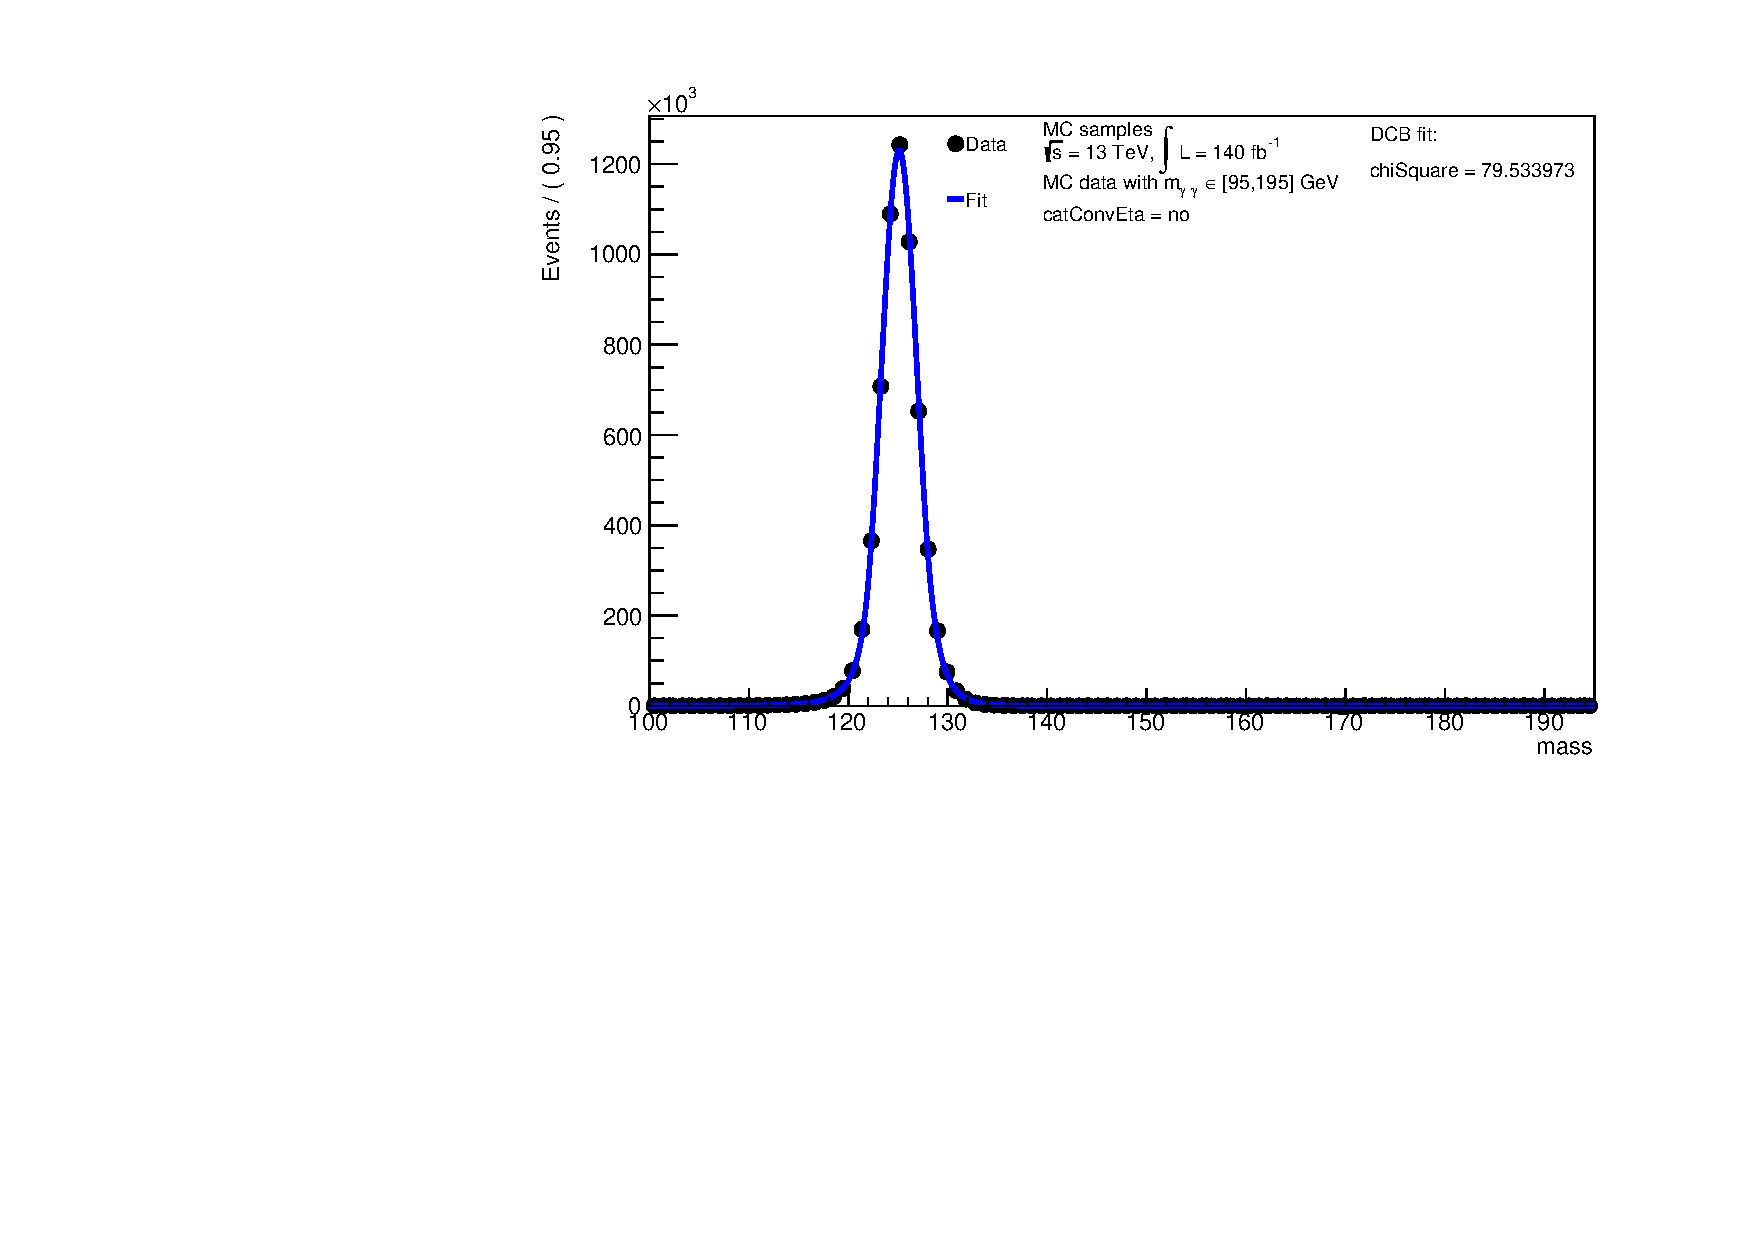
\includegraphics[width=.8\textwidth]{thesis_images/PowhegPy8_NNLOPS_ggH125_catConvEta_no_fit.pdf}
 					\caption{Signal fit using a simultaneous DSCB fit, for the resonance mass $m_X$ = 125 GeV and for the \texttt{Inclusive} categorisation.}
 					\label{fig:sig_fit}
 				\end{figure}
 				The signal shape is described by a Double-Sided Crystal Ball (DSCB) distribution (Figure \ref{fig:sig_fit}): this function has a gaussian core, which is useful to describe the mass of $H\to\gamma\gamma$ candidates, completed by power-law tails at lower and higher $m_{\gamma\gamma}$ values to account for experimental effects. Therefore the DSCB is described by 6 parameters: the mean $\mu$ and the standard deviation $\sigma$ of the Gaussian core and to 2 parameters for each polynomial tail ($a_{1,2}$,$p_{1,2}$). To create an analysis sensitive to additional spin-0 resonances, the signal model is build parametric in $m_X$ (\ref{appex:test}). Therefore, in the model, each DSCB parameter is inserted as a linear distribution of $m_X$, whose initial values are obtained from a linear fit on the 4 single DSCB fit parameters on the 4 different resonance mass MC (110, 125, 130 and 140 GeV)  (Figure \ref{fig:sigma_single}):
 				\begin{figure}
 					\centering
 					\includegraphics[width=.8\textwidth]{thesis_images/sigma_single.pdf}
 					\caption{The signal single DSCB fit $\sigma$ parameters for four different resonance mass MC samples fitted with a linear function of $m_X$.}
 					\label{fig:sigma_single}
 				\end{figure}
 				\begin{equation}\label{eq:DSCB_par}
 					p^{DSCB} = A_p + B_p\cdot m_X
 				\end{equation}
 				where $p^{DSCB}$ is a DSCB parameter. The $A_p$ and $B_p$ for each DSCB parameters in each category are obtained by a simultaneous fit to four different resonance masses (110, 125, 130 and 140 GeV) \textit{ggF} MC samples (Figure \ref{fig:sigma_fit}).
 				\begin{figure}
 					\centering
 					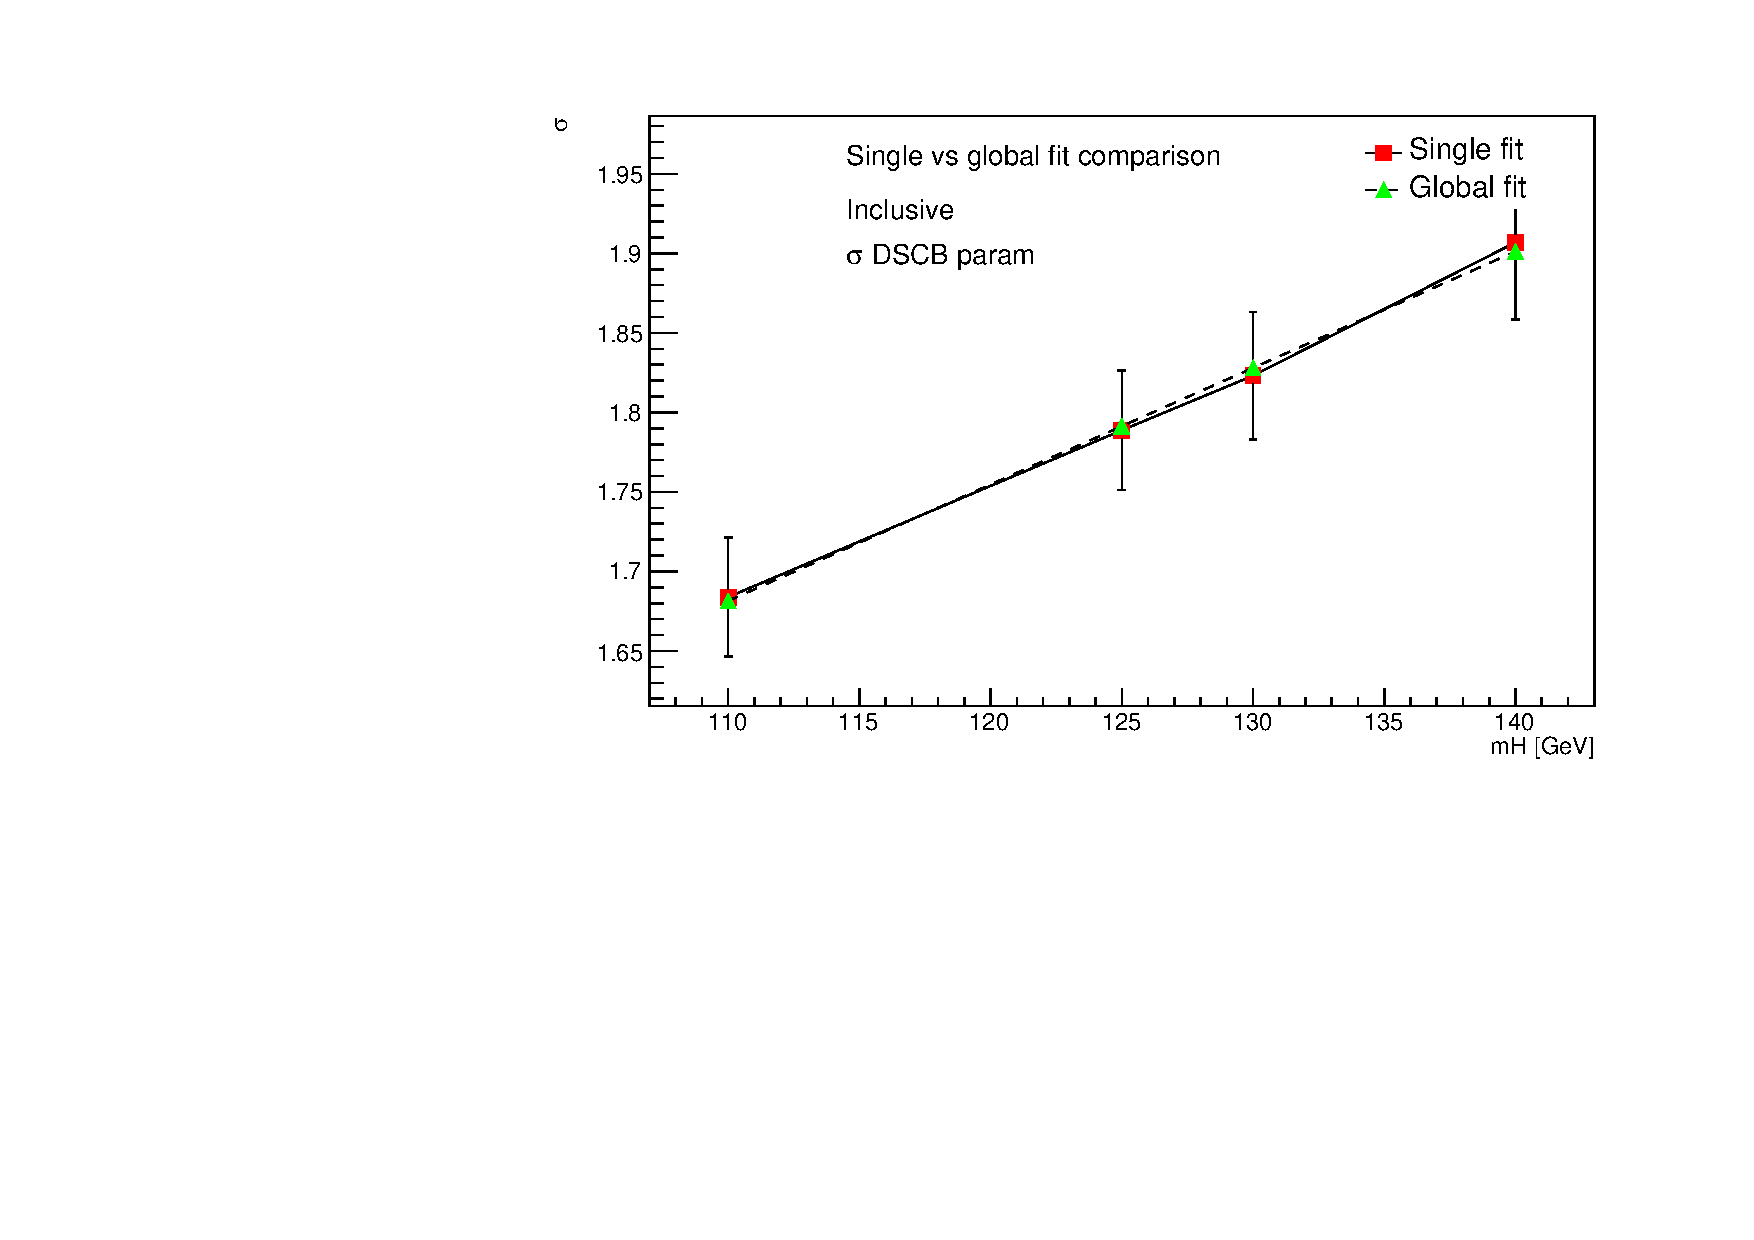
\includegraphics[width=.8\textwidth]{thesis_images/sigma_comp.pdf}
 					\caption{The signal simultaneous DSCB fit $\sigma$ parameter with a linear distribution of $m_X$ and single DSCB $\sigma$ parameter applied to four different resonance mass MC samples comparison for the \texttt{Inclusive} categorisation.}
 					\label{fig:sigma_fit}
 				\end{figure}
 				
 				
 				In each category $i$, the normalization of the signal pdf, called signal yield, is expressed as:
 				\begin{equation}\label{eq:signal_yield}
 					N^i = \sigma_{ggF}(m_X) \cdot A_X(m_X) \cdot Br_{\gamma\gamma}(m_X) \cdot \mathcal{L}_{Run2} \cdot C_X^i(m_X)
 				\end{equation}
 				where:
 				\begin{itemize}
 					\item $\sigma_{ggF}(m_X)$ is the cross-section value for the specific $m_X$ obtained by parametrising the $\sigma$ values for different masses \cite{yellow4}, showed in Figure \ref{fig:xs_fit}.
 					\item $A_X(m_X)$ is the acceptance value for the specific mass obtained from the linear fit of the four $A_X$ values for the four resonance masses showed in Figure \ref{fig:ax_fit}. The $A_X$ factor for each resonance mass is defined as the ratio of the number of events that pass the fiducial selection $n_{fid}$ and the total number of MC sample events $n_{all}$: $A_X = n_{fid}/n_{all}$.
 					\item $Br_{\gamma\gamma}(m_X)$ is the branching fraction value for the specific $m_X$ obtained by parametrising the $Br_{\gamma\gamma}$ values for different masses \cite{yellow3}, showed in Figure \ref{fig:br_fit}.  
 					\item $\mathcal{L}_{Run2}$ is the value of the luminosity of LHC Run2 and it is 140 fb$^{-1}$.
 					\item $C_X^i(m_X)$ for the specific mass is obtained from the linear fit of the four $C_X^i$ values for the four resonance masses showed in Figure \ref{fig:cx_fit}. $C_X$ is the ratio of the number of events that pass the selection after the reconstruction $n_{reco}$ and the number of those that pass the fiducial selection $n_{fid}$: $C_X = n_{reco}/n_{fid}$. The $C_X^i$ factors are calculated for each resonance mass and for each category $i$.
 				
 					\begin{figure}[h!]
 						\centering
 						\subfloat[$\sigma$ fit]{\includegraphics[width=.49\textwidth]{thesis_images/x_section_fit.pdf}\label{fig:xs_fit}}
 						\subfloat[$A_X$ fit]{\includegraphics[width=.49\textwidth]{thesis_images/ax_isFiducialMedium_linear_fit.pdf}\label{fig:ax_fit}}\\
 						\subfloat[$Br_{\gamma\gamma}$ fit]{\includegraphics[width=.49\textwidth]{thesis_images/br_fit.pdf}\label{fig:br_fit}}				
 						\subfloat[$C_X^i(m_X)$ fit for the \texttt{Inclusive} categorisation]{\includegraphics[width=.49\textwidth]{thesis_images/cx_fit_catConvEta_no.pdf}\label{fig:cx_fit}}	
 						\caption{Signal yield fit component for the \texttt{Inclusive} categorisation.}
 						\label{fig:signal_yiels}
 					\end{figure}
 				\end{itemize}
 				
 			\subsection{Non resonant background}
 				The non-resonant background in the $m_{\gamma\gamma}$ spectrum comes mainly from the non-resonant production of photon pairs ($\gamma\gamma$ events Figure \ref{fig:irr bkg}). Smaller background components come from events containing a photon and a jet ($\gamma j$ events) and events with two jets ($jj$ events), where the jets are misidentified as photons (Figure \ref{fig:rid bkg}). The study of background modelling in each category is performed on MC events normalized to data in dedicated sidebands ([100,110] and [170,195] GeV). The background in each category is approximated using \texttt{Sherpa} di-photon MC samples by fitting the $m_{\gamma\gamma}$ spectrum in the mass range [100,195] GeV with a selected model with free parameters of shape and normalisation. The fitting range is set wider than the blind search range ([110,170] GeV $m_X$) in order to have enough events in the $m_{\gamma\gamma}$ side-bands. This function form obtained using MC samples will be applied to data, determining the correct shape and normalisation.
 				
 				\begin{figure}[h]
 					\centering
 					\includegraphics[width=.8\textwidth]{thesis_images/bkg_100_195GeV_fit_catConvEta_no_prova.pdf}
 					\caption{Non-resonant background fit using the \ref{eq:bkg} function form for the \texttt{Inclusive} categorisation, using  \texttt{Sherpa} di-photon MC samples. The lower plot shows the ratio between the \texttt{Sherpa} di-photon MC distribution and the background fit applied on it.}
 					\label{fig:bkg_fit}
 				\end{figure}
 				The functional form used for the description of the non-resonant background in the $i$ category is (Figure \ref{fig:bkg_fit}):
 				\begin{equation}\label{eq:bkg}
 					f^i_{bkg}(m_{\gamma\gamma},N_{bkg}^i,a^i,b^i) = N_{bkg}^i\cdot\exp^{(a\cdot m_{\gamma\gamma}+b\cdot m_{\gamma\gamma}^2)}
 				\end{equation}
 				where $N_{bkg}^i$, which is the non-resonant background normalisation, $a^i$ and $b^i$ are free parameters for the specific $i$ category.
 				
 			\subsection{Higgs Standard Model background}
 				In order to investigate the presence of new spin-0 resonances, the SM Higgs$_{125}$ is included as a resonant background (HSM). The SM Higgs boson is described by a DSCB fit to HSM sample, which is obtained by merging all SM Higgs$_{125}$ production MC samples generated with a resonance mass $m_H=125$ GeV (Figure \ref{fig:HSM_fit}) Therefore for the $i$ category:
 				\begin{itemize}
 					\item the DSCB fit is applied to $i$ category HSM sample;
 					\item all DSCB parameters are fixed at their value after the fit and included in the analysis background shape;
 					\item the HSM background yield is obtained by counting the total number of events of $i$ category HSM sample (Table \ref{tab:HSM});
 				\end{itemize}  
 				Therefore, the HSM model has no free parameter, but they can be shifted due to the systematic experimental uncertainties that are included into the analysis, described in the next Section \ref{section:syst}
 				\begin{table}
 					\centering
						\begin{tabular}{lc}
							\toprule[1.5pt]
							Category &  HSM\_events \\
							\midrule
							Inclusive & 6232 \\
							\midrule
							catConvEta\_1 & 9601 \\
							catConvEta\_2 & 1601 \\
							catConvEta\_3 & 467 \\
							catConvEta\_4 & 599 \\
							catConvEta\_5 & 1821 \\
							catConvEta\_6 & 788 \\
							\midrule
							catConv\_1 & 3028 \\
							catConv\_2 & 3208 \\
							\bottomrule[1.5pt]
						\end{tabular}
 					\caption{Expected Number of SM Higgs$_{125}$ events for each category after selections.}
 					\label{tab:HSM}
 				\end{table}
 				\begin{figure}[]
 					\centering
 					\includegraphics[width=.8\textwidth]{thesis_images/bkg/HSM_fit_catConvEta_no.pdf}
 					\caption{SM Higgs$_{125}$ resonant background fit using a DSCB for the \texttt{Inclusive} categorisation.}
 					\label{fig:HSM_fit}
 				\end{figure}
 			
 			
 			
 			\subsection{Systematic uncertainties}\label{section:syst}
 				The systematic uncertainties are included into the likelihood model of the measurement as nuisance parameters. They arise from experimental sources and, for each category, they can be divided into two different groups: 
 				\begin{itemize}
 					\item uncertainties in the modelling of the $m_{\gamma\gamma}$ distribution for the signal and HSM models. They include the uncertainties in the energy resolution and scale of photon candidates. The photon energy scale uncertainties affect the peak position of the DSCB shape (Figure \ref{fig:scale_syst}) and they are calculated, following the procedure described in \cite{Aad_2019} as:
 					\begin{figure}
 						\centering
 						\includegraphics[width=.8\textwidth]{thesis_images/Syst/var_shape_scale_catConvEta_no.pdf}
 						\caption{Energy scale systematic uncertainty effect on the peak position of the DSCB shape, for the \texttt{Inclusive} categorisation.}
 						\label{fig:scale_syst}
 					\end{figure}
 					\begin{equation}\label{eq:shape_syst}
 						\delta\mu_c(\pm1\sigma)=\frac{<m_{\gamma\gamma}>_i(\pm1\sigma)}{<m_{\gamma\gamma}>_i} -1
 					\end{equation}
 					resulting in an impact of less than 0.5\%, depending on the category. The photon energy scale uncertainties are only applied to the signal model. The photon energy resolution uncertainties, which affect the Gaussian width of the DSCB shape (Figure \ref{fig:res_syst}), are calculated \cite{Aad_2019} as:
 					\begin{figure}
 						\centering
 						\includegraphics[width=.8\textwidth]{thesis_images/Syst/var_shape_res_catConvEta_no.pdf}
 						\caption{Energy resolution systematic uncertainty effect on the Gaussian width of the DSCB shape, for the \texttt{Inclusive} categorisation.}
 						\label{fig:res_syst}
 					\end{figure}
 					\begin{equation}\label{eq:res_syst}
 						\delta\sigma_c(\pm1\sigma)=\frac{IQR_i(\pm1\sigma)}{IQR_i}-1
 					\end{equation}
 					resulting in an impact of less than 12\%, depending on the category. $IQR$ is the InterQuartile Range of the distribution. The shape systematic uncertainties are reported in Table \ref{tab:shape}.
 					\begin{table}[tbp]
 						\centering
 						\resizebox{\textwidth}{!}{
							\begin{tabular}{lcccccc}
								\toprule[1.5pt]
								& \multicolumn{2}{c}{\small ATLAS\_EG\_RESOLUTION\_ALL$^{sig}$}
								& \multicolumn{2}{c}{\small ATLAS\_EG\_RESOLUTION\_ALL$^{HSM}$}	
								& \multicolumn{2}{c}{\small ATLAS\_EG\_SCALE\_ALL$^{sig}$}\\
								\midrule
								& \textbf{+1$\sigma$} & \textbf{-1$\sigma$}
								& \textbf{+1$\sigma$} & \textbf{-1$\sigma$}
								& \textbf{+1$\sigma$} & \textbf{-1$\sigma$}\\
								\cmidrule(lr){2-3} \cmidrule(lr){4-5} \cmidrule(lr){6-7}
								Inclusive 	  & 0.0841 & -0.0669 & 0.0865 & -0.0686 & 0.0043 & -0.0043 \\
								\midrule
								catConvEta\_1 & 0.0944 & -0.0511 & 0.0972 & -0.0522 & 0.0027 & -0.0027 \\
								catConvEta\_2 & 0.0899 & -0.0756 & 0.0923 & -0.0777 & 0.0051 & -0.0051 \\
								catConvEta\_3 & 0.1187 & -0.1164 & 0.1212 & -0.1187 & 0.0094 & -0.0094 \\
								catConvEta\_4 & 0.0795 & -0.0440 & 0.0824 & -0.0452 & 0.0029 & -0.0029 \\
								catConvEta\_5 & 0.0697 & -0.0608 & 0.0716 & -0.0623 & 0.0034 & -0.0034 \\
								catConvEta\_5 & 0.0781 & -0.0756 & 0.0801 & -0.0777 & 0.0052 & -0.0052 \\
								\midrule
								catConv\_1    & 0.0955 & -0.0731 & 0.0981 & -0.0749 & 0.0049 & -0.0049 \\
								catConv\_2    & 0.0733 & -0.0607 & 0.0754 & -0.0622 & 0.0037 & -0.0037 \\
								\bottomrule[1.5pt]
							\end{tabular}
						}
 						\caption{Signal and HSM $\pm1\sigma$ variations for Resolution and Scale shape systematic uncertainties for each category.}
 						\label{tab:shape}
 					\end{table}
 					\item uncertainties in the expected signal and HSM yields. They include: the impact of the photon energy scale and resolution uncertainties on the selection efficiency \cite{Aad_2019}, the photon identification and isolation efficiencies \cite{Aad_2019}, the efficiency of the diphoton trigger \cite{e_trigger} and the modelling of pile-up in the simulation. All these systematic uncertainties have an impact of less than 2\% (Figure \ref{fig:yield_syst}). Since the analysis shown not rely on SM production modes fractions, the signal yield is also affected by the production mode dependence. For each category the values of $C_{X\ prod}$ are extracted from the available MC samples for each production mode and parametrised as functions of the mass. For each category the other production mode systematic uncertainty is the maximum of  $$\dfrac{|C^{fit}_{X\ prod}-C^{fit}_{X\ ggF}|}{C^{fit}_{X\ ggF}}$$ by varying production modes and resonance mass (110,125,130,140 GeV) (Figure \ref{fig:prod_mode_syst}). The impact of this systematic uncertainty for each category is reported in the Table \ref{tab:prod_mode}.
 					\begin{center}
 						\begin{figure}
 							\centering
 							\includegraphics[width=.8\textwidth]{thesis_images/Syst/var_catConvEta_no_sig_fid.pdf}
 							\caption{Signal yield systematic uncertainties for the \texttt{Inclusive} categorisation.}
 							\label{fig:yield_syst}
 						\end{figure}
 						\begin{figure}
 							\centering
 							\includegraphics[width=.8\textwidth]{thesis_images/Signal/cx_all_prod_catConvEta_no.pdf}
 							\caption{Four different resonance mass MC samples $C_X$ parameters fitted with a linear distribution of $m_X$, for different production modes and for the \texttt{Inclusive} categorisation.}
 							\label{fig:prod_mode_syst}
 						\end{figure}
 						\begin{table}[tbp]
 							\centering
 							\begin{tabular}{lc}
 								\toprule[1.5pt]
 								Category		& $\sigma^{prod\ modes}$	\\
 								\midrule
 								Inclusive		& 0.044				\\
 								\midrule
 								catConvEta\_1 	& 0.307				\\
 								catConvEta\_2 	& 0.028				\\
 								catConvEta\_3 	& 0.144				\\
 								catConvEta\_4 	& 0.324				\\
 								catConvEta\_5 	& 0.048				\\
 								catConvEta\_6 	& 0.153				\\
 								\midrule
 								catConv\_1 		& 0.074				\\
 								catConv\_2 		& 0.037				\\
 								\bottomrule[1.5pt]
 							\end{tabular}
 							\caption{Relative systematic uncertainties on the signal yields due to the different production modes for each category.}
 							\label{tab:prod_mode}
 						\end{table}
 					\end{center}
 				\end{itemize} 
 			\begin{center}
 				\begin{table}[tbp]
 					\centering
 					\begin{tabular}{lcc}
 						\toprule[1.5pt]
 						Systematic uncertainty					& Signal model	& HSM model	\\
 						\midrule
 						ATLAS\_EG\_RESOLUTION\_ALL				& $\ast$		& 			\\
 						ATLAS\_EG\_SCALE\_ALL					& $\ast$		& $\ast$	\\
 						\midrule
 						ATLAS\_EG\_RESOLUTION\_ALL				& $\ast$		& $\ast$	\\
 						ATLAS\_EG\_SCALE\_ALL					& $\ast$		& $\ast$	\\
 						ATLAS\_PH\_EFF\_ID\_Uncertainty			& $\ast$		& $\ast$	\\
 						ATLAS\_PH\_EFF\_ISO\_Uncertainty		& $\ast$		& $\ast$	\\
 						ATLAS\_PH\_EFF\_TRIGGER\_Uncertainty	& $\ast$		& $\ast$	\\
 						ATLAS\_PRW\_DATASF						& $\ast$		& $\ast$	\\
 						ATLAS\_prod\_modes						& $\ast$		& 			\\
 						\bottomrule[1.5pt]
 					\end{tabular}
 					\caption{List of the systematic uncertainties of the signal and HSM models.}
 					\label{tab:sig_HSM_syst}
 				\end{table}
 			\end{center}
 			\vspace{-2.cm}
 			The signal and HSM systematic uncertainties are reported in Table \ref{tab:sig_HSM_syst}.
 			
 			
 				
 				
 		\section{Results}
 			Once the categorisations and models are constructed they can be tested on a MC sample of signal and background events representing the data expectation. The performances for each category, without the systematic uncertainties, can firstly evaluated looking at the $\sigma^{DSCB}$ of the Double Side Crystal Ball fit. Since the aim of the categorisation is to maximise the signal over background (S/B) ratio and thus provide an analysis as sensitive to new spin-0 resonances as possible, a good categorisation should isolate events with a $\sigma^{DSCB}$ on MC signal events smaller then the one of the benchmark category, which in thesis is the \texttt{Inclusive}. The $\sigma^{DSCB}$ of \texttt{Inclusive}, \texttt{catConvEta} and \texttt{catConv} categorisations for the signal models are reported in Table \ref{tab:sigma}.
 			\begin{table}[tbp]
 				\centering
 				\begin{tabular}{lcccc}
 					\toprule[1.5pt]
 					Category		& $\sigma^{DSCB}_{110 GeV}$	& $\sigma^{DSCB}_{125 GeV}$	& $\sigma^{DSCB}_{130 GeV}$ 	& $\sigma^{DSCB}_{140 GeV}$ 	\\
 					\midrule
 					Inclusive 		& 1.681 	& 1.791 	& 1.828 	& 1.902	\\ 
 					\midrule
 					catConvEta\_1 	& 1.381 	& 1.476 	& 1.508 	& 1.571 	\\
 					catConvEta\_2 	& 1.600 	& 1.709  	& 1.746 	& 1.818 	\\ 
 					catConvEta\_3 	& 1.889 	& 2.061 	& 2.119 	& 2.233 	\\ 
 					catConvEta\_4 	& 1.518 	& 1.614 	& 1.645 	& 1.709 	\\ 
 					catConvEta\_5 	& 1.866 	& 1.971 	& 2.005 	& 2.075 	\\ 
 					catConvEta\_6 	& 2.206 	& 2.409 	& 2.477 	& 2.613 	\\
 					\midrule 
 					catConv\_1 		& 1.559 	& 1.661 	& 1.696 	& 1.764 	\\
 					catConv\_2 		& 1.845 	& 1.958 	& 1.996 	& 2.072 	\\
 					\bottomrule[1.5pt]
 				\end{tabular}
 				\caption{Signal $\sigma^{DSCB}$ for each category obtained by fitting four different $m_X$ MC samples (110, 125, 130 and 140 GeV).}
 				\label{tab:sigma}
 			\end{table}
 			One can see how some categories exhibit a better resolution than the \texttt{Inclusive} category, for example \texttt{catConvEta\_1}, \texttt{catConvEta\_4} or \texttt{catConv\_1}. Another preliminary categorisation performance test is to look at their significances, defined as the ratio of the signal events number and the square root of the non resonant background events number ($Sig/\sqrt{Bkg}$). Only events falling in  a $\pm3\sigma$ window around the peak of the signal distribution are counted. The significances of each categorisation are obtained as square sum of the single category significance, their values are reported in Table \ref{tab:signif}. One can notice that the \texttt{catConvEta} categorisation is able to bring a $\sim$2\% improvement in significance compared to the \texttt{Inclusive} case, whereas \texttt{catConv} categorisation improvement is negligible ($\sim$0.3\%) or even negative. 
 			\begin{table}[tbp]
 				\resizebox{\textwidth}{!}{
	 				\centering
	 				\begin{tabular}{lcccc}
	 					\toprule[1.5pt]
	 					Category		& $Sig/\sqrt{Bkg}_{110 GeV}$	& $Sig/\sqrt{Bkg}_{125 GeV}$	& $Sig/\sqrt{Bkg}_{130 GeV}$ 	& $Sig/\sqrt{Bkg}_{140 GeV}$ 	\\
	 					\midrule
	 					Inclusive 		& 8.974	 & 11.893 & 11.832 & 9.246 \\
	 					\midrule
	 					catConvEta\_1 	& 4.559	& 6.065 & 6.046 & 4.795 	\\
	 					catConvEta\_2 	& 4.557	& 5.989 & 6.022 & 4.702 	\\
	 					catConvEta\_3 	& 2.259	& 2.907 & 2.866 & 2.241 \\ 
	 					catConvEta\_4	& 3.380 & 4.540	& 4.495 & 3.594 \\
	 					catConvEta\_5 	& 4.341	& 5.764 & 5.732 & 4.504 \\ 
	 					catConvEta\_6 	& 2.652 & 3.441 & 3.413 & 2.673 \\
	 					catConvEta Sum	& 9.162 & 12.114 & 12.071 & 9.511 \\
	 					\midrule 
	 					catConv\_1 		& 6.657 & 8.773	& 8.781 & 6.902 \\ 
	 					catConv\_2 		& 6.018 & 7.914 & 7.860 & 6.195 \\
	 					catConv Sum 	& 8.974 & 11.815 & 11.785 & 9.274	\\
	 					\bottomrule[1.5pt]
	 				\end{tabular}
 				}
 				\caption{Significances for each category defined as the ratio of the signal events number and the square root of the non resonant background events number ($Sig/\sqrt{Bkg}$) in to a $\pm3\sigma$ window around the peak. Four different $m_X$ MC samples (110, 125, 130 and 140 GeV) are studied. For each categorisation the sum in quadrature of the significances of all categories is reported.}
 				\label{tab:signif}
 			\end{table}
 			
 			Given the promising improvement obtained with the proposed categorisation, a complete study of the performances without the impact of the systematic uncertainties is performed comparing the expected  $p_0$ values (Figure \ref{fig:p0_res_inc}). They are obtained generating an Asimov dataset for each resonance mass $m_X$ with $\mu$=1, and then calculating the local $p_0$ value, thus estimating the maximum capacity to detect a signal. %Since $p_0$ is being calculated with m$_X$ corresponding to the peak of the Asimov dataset, the effect of systematic uncertainties is zero, as the model is able to perfectly reproduce the distribution. $\sim$6.3\% ($\sim$1.2\%)
 			Looking at the values reported in Table \ref{tab:p0_imp}, \texttt{catConvEta} categorisation  is able to bring about $\sim$6.3\% improvement in discovery capability, whereas \texttt{catConv} categorisation is able to bring about a $\sim$1.2\% improvement (without the systematics). 
 			%The expected  $p_0$ values and observed ones obtained by using Asimov dataset with $\mu$=1 and m$_X$ = 125 (140) GeV, for the different categorisation are showed in Figure \ref{fig:p0}. 
 			A comparison of the different categorisation expected $p_0$ is shown in Figure \ref{fig:p0_comp}. A signal significance ranging from few $\sigma$ to $\sim12\sigma$ can be achieved in the search for new spin-0 resonance in the [110,170] GeV $m_X$ mass range, assuming mass dependence of the cross-section.  When no systematic uncertainties are included in the fit, \texttt{catConvEta} (\texttt{catConv}) categorisation also results in a $\sim$7.6\% ($\sim$2.4\%) enhancement in limits setting (Figure \ref{fig:limits_comp}), compared to \texttt{Inclusive} category, whose limits are shown in Figure \ref{fig:limit_HSM_inc}.
 			\begin{table}[tbp]
				\centering
				\begin{tabular}{lcc}
					\toprule[1.5pt]
					Category 			& Minimum expected $p_0$ 	& Significance		\\
					\midrule
					\texttt{Inclusive}	& 3.556e-30					& 11.343$\sigma$	\\
					\texttt{catConvEta}	& 8.547e-34					& 12.061$\sigma$	\\
					\texttt{catConv}	& 7.956e-31					& 11.483$\sigma$ 	\\
					\bottomrule[1.5pt]
				\end{tabular}
 				\caption{Minimum expected $p_0$ for $m_X$ = 131 GeV and its significance values for each categorisation.}
 				\label{tab:p0_imp}
 			\end{table}
 			\begin{figure}
 				\centering
 				\includegraphics[width=.8\textwidth]{thesis_images/p0_no_catConvEta.pdf}
 				\caption{Expected $p_0$ values and observed ones values obtained by using Asimov dataset with $\mu$=1 and $m_X$ = 125 (140) GeV, for the \texttt{Inclusive} categorisation, as a function of $m_X$.}
 				\label{fig:p0_res_inc}
 			\end{figure}
 			\begin{figure}
 				\centering
 				\includegraphics[width=.8\textwidth]{thesis_images/p0_exp_imp.pdf}
 				\caption{Expected $p0$ as a function of $m_X$ for \texttt{Inclusive}, \texttt{catConvEta} and \texttt{catConv} categorisations.}
 				\label{fig:p0_comp}
 			\end{figure}
 			\begin{figure}
 				\centering
 				\includegraphics[width=.8\textwidth]{thesis_images/imp_nom_gaus.pdf}
 				\caption{\texttt{catConvEta} and \texttt{catConv} categorisation improvement in the 95\% CL$_S$ upper limits with \texttt{Inclusive} category as reference, as function of $m_X$.}
 				\label{fig:limits_comp}
 			\end{figure}
 			\begin{figure}
 				\centering
 				\includegraphics[width=.8\textwidth]{thesis_images/plot_AsimovData_0_ggHyy_MC_no_catConvEta_syst_HSM_fid_nom_gaus.pdf}
 				\caption{95\% CL$_S$ upper limits plots for \texttt{Inclusive} categorisation, as a function of $m_X$.}
 				\label{fig:limit_HSM_inc}
 			\end{figure}
 			%To observe the effect of systematic uncertainties, one can instead look at the minimum observed $p_0$ values obtained by using Asimov dataset with $\mu$=1 and m$_X$ = 125 (140) GeV, reported in Table 56. \texttt{catConvEta} categorisation brings an improvement of $\sim$2 ($\sim$3) orders of magnitude whereas \texttt{catConv} one by a factor of 5 for m$_X$ = 125 GeV. The \texttt{catConv} categories discovery performance at m$_X$ is worse than the \texttt{Inclusive} categorisation.
 			Translating the expected signal strength into a fiducial cross section, which is a cross section for the subset of a process in which the distinctive process signatures are visible within the sensitive regions of the detector volume (the \textit{Fiducial} volume), the performance of the categorisation is also checked on $\sigma^{fid}$ limits setting. The impact of the systematic uncertainties is also quantified. At $m_X$ = 125 GeV, the \texttt{catConvEta} exclusion performance is $\sim$1.5\% better then \texttt{Inclusive}, whereas \texttt{catConv} categorisation brings a small improvement of $\sim$0.3\%. The maximum difference in the limits with \texttt{Inclusive} as reference is $\sim$4.2\% for \texttt{catConvEta} and $\sim$2\% for \texttt{catConv} at $m_X$ = 170 GeV (Figure \ref{fig:limits_comp}). In the [110,170] GeV $m_X$ mass range, the excluded fiducial cross-section for a signal ranges from $\sim 3.4$ pb to $\sim 34.6$ pb depending on the new resonance mass. 
 			
 			
 			
 			
	\chapter{Conclusions}\label{chapter:5}
		The potential search for new resonances in the 110 to 170 GeV diphoton invariant mass range using 140 fb$^{-1}$ of $pp$ collisions collected at $\sqrt{s}$=13 TeV with the ATLAS detector has been presented.
		%performed in this thesis, led to the creation of a model defined as a function of the resonance mass $m_X$. This need arises as this analysis is looking for new physics, therefore a model independent of the Standard Model must be created. 
		
		
		%Using events with pairs of high-$p_T$ and isolated photons, which are classified into mutually exclusive categories designed to enhance the analysis sensitivity, the model is created. Three different type of categorisations are tested and compared: \texttt{Inclusive} (no selections applied), \texttt{catConvEta} ($\gamma$ conversions and $\eta$  selections applied) and \texttt{catConvEta} (only $\gamma$ conversions selections applied). Using these three categorisations, three different analysis models are created. This distribution in each category is describedby an extended probability density function (pdf) in which the signal and backgroundsshapes are analytic functions of m γγ .The results of this thesis are about the signal modelling as function of $m_X$ and the categorisation working point. 
		
		The analysis is based on the selection of pairs of high-$p_T$ and isolated photons. The events are classified into mutually exclusive categories designed to enhance the analysis sensitivity. Three different types of categorisations are tested and compared with each other: \texttt{Inclusive} (no selections applied), \texttt{catConvEta} ($\gamma$ conversions and $\eta$  selections applied) and \texttt{catConvEta} (only $\gamma$ conversions selections applied). The signal model in each category is parametrised as a function of the mass of the resonance and it is obtained from applying a simultaneous Double-Side Crystal Ball fit on different simulated MC samples of SM (spin0) Higgs bosons decaying into two photons. To reduce the dependence of the model from SM assumptions only \textit{ggF} samples are used. The differences in efficiency from the other production modes are included as systematic uncertainties. This background in each category is described by a smoothly falling function whose normalization and shape parameters will be determined from data. In order to investigate the presence of new spin-0 resonances, the SM Higgs 125 is also included as background. 
		
		A combined maximum likelihood fit in all the categories is performed to investigate the presence of a signal by computing the compatibility of the observed data with the background-only hypothesis $p_0$ \cite{Statistic} and assessing limits \cite{Statistic} on the fiducial production cross-section in case no excess of signal is observed. Looking at limits on the signal cross-section for different categorisations, the analysis strategy is selected as the best trade-off analysis performances and SM independence. A more detailed categorisation allows to improve the analysis sensitivity from the statistical point of view, however detailed categorisations generally introduce a larger systematic uncertainty due to model dependence. The best categorisation has been found to be the \texttt{catConvEta} that shows an always positive improvement in the exclusion performances, which reaches its maximum value 4.2\% at $m_X$ = 170 GeV, compared to the \textit{Inclusive} one. On the contrary, the \texttt{catConv} categorisation should be discarded as it is not able to bring a consistently positive improvement on the limits compared to \texttt{Inclusive} over the $m_{\gamma\gamma}$ range, and its performances are inferior to \texttt{catConvEta}. Therefore using the \texttt{catConvEta} categorisation the analysis shows that in the [110,170] GeV $m_X$ mass range:
		\begin{itemize}
			\item a signal significance ranging from few $\sigma$ to $\sim12\sigma$ can be achieved in the search for new spin-0 resonance, assuming the SM mass dependence of the cross-section;
			\item the excluded fiducial cross-section for a signal ranges from $\sim 3.4$ pb to $\sim 34.6$ pb depending on the new resonance mass.
		\end{itemize}
		
		In conclusion, the potential of search for new resonances in [105,200] $m_{\gamma\gamma}$ range using 140 fb$^{-1}$ of $pp$ collisions collected at $\sqrt{s}$=13 TeV with the ATLAS detector, has been investigated in this thesis. The best categorisation obtained from the trade-off between performances and SM independence is \texttt{catConvEta}. The analysis is still blind so no results based on data have been shown. The results presented in this thesis represent the first step towards the unblinding.
		
		
		
		%In conclusion, the search for new resonances in [105,200] $m_{\gamma\gamma}$ range using 140 fb$^{-1}$ of $pp$ collisions collected at $\sqrt{s}$=13 TeV with the ATLAS detector, performed in this thesis showed that it is possible to created perfectly functioning signal model as function of the resonance mass $m_X$. Another important result of this analysis is that the best categorisation obtained from the trade-off between performances and model SM independence is \texttt{catConvEta}. Therefore this configuration should be the starting point for further development of the analysis, such as the spurious signal study or, once completed, its application to ATLAS observed data. 
 			
 			
	\appendix
	\chapter{Signal model}
		\begin{figure}[h!]
			\centering
			\subfloat[\texttt{catConv\_1}]
			{\includegraphics[width=.49\textwidth]{thesis_images/Signal/PowhegPy8_NNLOPS_ggH125_catConv_1_fit_prova.pdf}\label{fig:sig_conv_1}}		
			\subfloat[\texttt{catConv\_2}]
			{\includegraphics[width=.49\textwidth]{thesis_images/Signal/PowhegPy8_NNLOPS_ggH125_catConv_2_fit_prova.pdf}\label{fig:sig_conv_2}}	
			\caption{Signal fit using a simultaneous DSCB fit, for the resonance mass $m_X$ = 125 GeV and for the \texttt{catConv} categorisation.}
			\label{fig:sig_conv}
		\end{figure}
		\begin{figure}[h!]
			\centering
			\subfloat[\texttt{catConvEta\_1}]
			{\includegraphics[width=.49\textwidth]{thesis_images/Signal/PowhegPy8_NNLOPS_ggH125_catConvEta_1_fit_prova.pdf}\label{fig:sig_eta_1}}		
			\subfloat[\texttt{catConvEta\_2}]
			{\includegraphics[width=.49\textwidth]{thesis_images/Signal/PowhegPy8_NNLOPS_ggH125_catConvEta_2_fit_prova.pdf}\label{fig:sig_eta_2}}\\
			\subfloat[\texttt{catConvEta\_3}]
			{\includegraphics[width=.49\textwidth]{thesis_images/Signal/PowhegPy8_NNLOPS_ggH125_catConvEta_3_fit_prova.pdf}\label{fig:sig_eta_3}}		
			\subfloat[\texttt{catConvEta\_4}]
			{\includegraphics[width=.49\textwidth]{thesis_images/Signal/PowhegPy8_NNLOPS_ggH125_catConvEta_4_fit_prova.pdf}\label{fig:sig_eta_4}}\\
			\subfloat[\texttt{catConvEta\_5}]
			{\includegraphics[width=.49\textwidth]{thesis_images/Signal/PowhegPy8_NNLOPS_ggH125_catConvEta_5_fit_prova.pdf}\label{fig:sig_eta_5}}		
			\subfloat[\texttt{catConvEta\_6}]
			{\includegraphics[width=.49\textwidth]{thesis_images/Signal/PowhegPy8_NNLOPS_ggH125_catConvEta_6_fit_prova.pdf}\label{fig:sig_eta_6}}
			\caption{Signal fit using a simultaneous DSCB fit, for the resonance mass $m_X$ = 125 GeV and for the \texttt{catConvEta} categorisation.}
			\label{fig:sig_eta}
		\end{figure}
	
	\chapter{New resonances sensitivity of the signal model test}\label{appex:test}
		The signal model as a function of the resonance mass is tested in order to verify its capability to describe a signal with a mass not used in the fit. Therefore a test signal model is created with a simultaneous Double Side Crystal Ball fit applied on only \textit{ggF} 110, 130 and 140 GeV MC samples. Then this model is applied to the MC 125 GeV sample, which in this case simulates a new resonance. As shown in Figure \ref{fig:sig_test}, the model is able to fit correctly the MC 125 GeV sample, so signal model as a function of resonant mass is sensible to new resonances.
		\vspace{.5cm}
		\begin{figure}[h!]
			\centering
			\includegraphics[width=.7\textwidth]{thesis_images/sig_test.png}
			\caption{Test signal model created using a simultaneous DSCB fit on \textit{ggF} 110, 130 and 140 GeV MC samples, applied to the MC 125 GeV sample, for the \texttt{Inclusive} categorisation.}
			\label{fig:sig_test}
		\end{figure}
		
	\chapter{Non-resonant background model}
		\begin{figure}[h!]
			\centering
			\subfloat[\texttt{catConv\_1}]
			{\includegraphics[width=.49\textwidth]{thesis_images/bkg/bkg_100_195GeV_fit_catConv_1_prova.pdf}\label{fig:bkg_conv_1}}		
			\subfloat[\texttt{catConv\_2}]
			{\includegraphics[width=.49\textwidth]{thesis_images/bkg/bkg_100_195GeV_fit_catConv_2_prova.pdf}\label{fig:bkg_conv_2}}	
			\caption{Non-resonant background fit using the \ref{eq:bkg} function form for the \texttt{catConv} categorisation, using  \texttt{Sherpa} di-photon MC samples. The lower plot shows the ratio between the \texttt{Sherpa} di-photon MC distribution and the background fit applied on it.}
			\label{fig:bkg_conv}
		\end{figure}
		\begin{figure}[h!]
			\centering
			\subfloat[\texttt{catConvEta\_1}]
			{\includegraphics[width=.49\textwidth]{thesis_images/bkg/bkg_100_195GeV_fit_catConvEta_1_prova.pdf}\label{fig:bkg_eta_1}}		
			\subfloat[\texttt{catConvEta\_2}]
			{\includegraphics[width=.49\textwidth]{thesis_images/bkg/bkg_100_195GeV_fit_catConvEta_2_prova.pdf}\label{fig:bkg_eta_2}}\\
			\subfloat[\texttt{catConvEta\_3}]
			{\includegraphics[width=.49\textwidth]{thesis_images/bkg/bkg_100_195GeV_fit_catConvEta_3_prova.pdf}\label{fig:bkg_eta_3}}		
			\subfloat[\texttt{catConvEta\_4}]
			{\includegraphics[width=.49\textwidth]{thesis_images/bkg/bkg_100_195GeV_fit_catConvEta_4_prova.pdf}\label{fig:bkg_eta_4}}\\
			\subfloat[\texttt{catConvEta\_5}]
			{\includegraphics[width=.49\textwidth]{thesis_images/bkg/bkg_100_195GeV_fit_catConvEta_5_prova.pdf}\label{fig:bkg_eta_5}}		
			\subfloat[\texttt{catConvEta\_6}]
			{\includegraphics[width=.49\textwidth]{thesis_images/bkg/bkg_100_195GeV_fit_catConvEta_6_prova.pdf}\label{fig:bkg_eta_6}}
			\caption{Non-resonant background fit using the \ref{eq:bkg} function form for the \texttt{catConvEta} categorisation, using  \texttt{Sherpa} di-photon MC samples. The lower plot shows the ratio between the \texttt{Sherpa} di-photon MC distribution and the background fit applied on it.}
			\label{fig:bkg_eta}
		\end{figure}
	
	\chapter{SM Higgs boson background model}
		\begin{figure}[h!]
			\centering
			\subfloat[\texttt{catConv\_1}]
			{\includegraphics[width=.49\textwidth]{thesis_images/bkg/HSM_fit_catConv_1.pdf}\label{fig:HSM_conv_1}}		
			\subfloat[\texttt{catConv\_2}]
			{\includegraphics[width=.49\textwidth]{thesis_images/bkg/HSM_fit_catConv_2.pdf}\label{fig:HSM_conv_2}}	
			\caption{SM Higgs$_{125}$ resonant background fit using a DSCB for the \texttt{catConv} categorisation}
			\label{fig:HSM_conv}
		\end{figure}
		\begin{figure}[h!]
			\centering
			\subfloat[\texttt{catConvEta\_1}]
			{\includegraphics[width=.49\textwidth]{thesis_images/bkg/HSM_fit_catConvEta_1.pdf}\label{fig:HSM_eta_1}}		
			\subfloat[\texttt{catConvEta\_2}]
			{\includegraphics[width=.49\textwidth]{thesis_images/bkg/HSM_fit_catConvEta_2.pdf}\label{fig:HSM_eta_2}}\\
			\subfloat[\texttt{catConvEta\_3}]
			{\includegraphics[width=.49\textwidth]{thesis_images/bkg/HSM_fit_catConvEta_3.pdf}\label{fig:HSM_eta_3}}		
			\subfloat[\texttt{catConvEta\_4}]
			{\includegraphics[width=.49\textwidth]{thesis_images/bkg/HSM_fit_catConvEta_4.pdf}\label{fig:HSM_eta_4}}\\
			\subfloat[\texttt{catConvEta\_5}]
			{\includegraphics[width=.49\textwidth]{thesis_images/bkg/HSM_fit_catConvEta_5.pdf}\label{fig:HSM_eta_5}}		
			\subfloat[\texttt{catConvEta\_6}]
			{\includegraphics[width=.49\textwidth]{thesis_images/bkg/HSM_fit_catConvEta_6.pdf}\label{fig:HSM_eta_6}}
			\caption{SM Higgs$_{125}$ resonant background fit using a DSCB for the \texttt{catConvEta} categorisation}
			\label{fig:HSM_eta}
		\end{figure}
	
	\chapter{Signal yield systematic uncertainty}
		\begin{figure}[h!]
			\centering
			\subfloat[\texttt{catConv\_1}]
			{\includegraphics[width=.49\textwidth]{thesis_images/Syst/var_catConv_1_sig_fid.pdf}\label{fig:ysig_conv_1}}		
			\subfloat[\texttt{catConv\_2}]
			{\includegraphics[width=.49\textwidth]{thesis_images/Syst/var_catConv_2_sig_fid.pdf}\label{fig:ysig_conv_2}}	
			\caption{Signal yield systematic uncertainties for the \texttt{catConv} categorisation.}
			\label{fig:ysig_conv}
		\end{figure}
		\begin{figure}[h!]
			\centering
			\subfloat[\texttt{catConvEta\_1}]
			{\includegraphics[width=.49\textwidth]{thesis_images/Syst/var_catConvEta_1_sig_fid.pdf}\label{fig:ysig_eta_1}}		
			\subfloat[\texttt{catConvEta\_2}]
			{\includegraphics[width=.49\textwidth]{thesis_images/Syst/var_catConvEta_2_sig_fid.pdf}\label{fig:ysig_eta_2}}\\
			\subfloat[\texttt{catConvEta\_3}]
			{\includegraphics[width=.49\textwidth]{thesis_images/Syst/var_catConvEta_3_sig_fid.pdf}\label{fig:ysig_eta_3}}		
			\subfloat[\texttt{catConvEta\_4}]
			{\includegraphics[width=.49\textwidth]{thesis_images/Syst/var_catConvEta_4_sig_fid.pdf}\label{fig:ysig_eta_4}}\\
			\subfloat[\texttt{catConvEta\_5}]
			{\includegraphics[width=.49\textwidth]{thesis_images/Syst/var_catConvEta_5_sig_fid.pdf}\label{fig:ysig_eta_5}}		
			\subfloat[\texttt{catConvEta\_6}]
			{\includegraphics[width=.49\textwidth]{thesis_images/Syst/var_catConvEta_6_sig_fid.pdf}\label{fig:ysig_eta_6}}
			\caption{Signal yield systematic uncertainties for the \texttt{catConvEta} categorisation.}
			\label{fig:ysig_eta}
		\end{figure}

	\chapter{SM Higgs boson yield systematic uncertainty}
		\begin{figure}[h!]
			\centering
			\subfloat[\texttt{catConv\_1}]
			{\includegraphics[width=.49\textwidth]{thesis_images/Syst/var_catConv_1_HSM.pdf}\label{fig:yHSM_conv_1}}		
			\subfloat[\texttt{catConv\_2}]
			{\includegraphics[width=.49\textwidth]{thesis_images/Syst/var_catConv_2_HSM.pdf}\label{fig:yHSM_conv_2}}	
			\caption{SM Higgs boson yield systematic uncertainties for the \texttt{catConv} categorisation.}
			\label{fig:yHSM_conv}
		\end{figure}
		\begin{figure}[h!]
			\centering
			\subfloat[\texttt{catConvEta\_1}]
			{\includegraphics[width=.49\textwidth]{thesis_images/Syst/var_catConvEta_1_HSM.pdf}\label{fig:yHSM_eta_1}}		
			\subfloat[\texttt{catConvEta\_2}]
			{\includegraphics[width=.49\textwidth]{thesis_images/Syst/var_catConvEta_2_HSM.pdf}\label{fig:yHSM_eta_2}}\\
			\subfloat[\texttt{catConvEta\_3}]
			{\includegraphics[width=.49\textwidth]{thesis_images/Syst/var_catConvEta_3_HSM.pdf}\label{fig:yHSM_eta_3}}		
			\subfloat[\texttt{catConvEta\_4}]
			{\includegraphics[width=.49\textwidth]{thesis_images/Syst/var_catConvEta_4_HSM.pdf}\label{fig:yHSM_eta_4}}\\
			\subfloat[\texttt{catConvEta\_5}]
			{\includegraphics[width=.49\textwidth]{thesis_images/Syst/var_catConvEta_5_HSM.pdf}\label{fig:yHSM_eta_5}}		
			\subfloat[\texttt{catConvEta\_6}]
			{\includegraphics[width=.49\textwidth]{thesis_images/Syst/var_catConvEta_6_HSM.pdf}\label{fig:yHSM_eta_6}}
			\caption{SM Higgs boson yield systematic uncertainties for the \texttt{catConvEta} categorisation.}
			\label{fig:yHSM_eta}
		\end{figure}
	
	\chapter{Run1 mass categorisation}\label{appex:Run1}
		The Run1 mass categorisation used for the 125 GeV Standard Model Higgs boson discovery is based on $\gamma$ conversion status, $\eta$ position and  $p_{Tt_{\gamma\gamma}}$ momentum selections. It can not be used in this analysis since it has an enormous impact on the model dependence, as reported in Table \ref{tab:Run1}.
		\begin{table}[htbp]
			\begin{center}
				\begin{tabular}{lc}
					\toprule[1.5pt]
					Category			& $\sigma^{prod\ modes}$	\\
					\midrule
					Inclusive			& 0.044				\\
					\midrule
					catMass\_Run1\_1 	& 0.440				\\
					catMass\_Run1\_2 	& 5.972				\\
					catMass\_Run1\_3 	& 0.512				\\
					catMass\_Run1\_4 	& 4.116				\\
					catMass\_Run1\_5 	& 0.144				\\
					catMass\_Run1\_6 	& 0.438				\\
					catMass\_Run1\_7 	& 5.788				\\
					catMass\_Run1\_8 	& 0.533				\\
					catMass\_Run1\_9 	& 4.008				\\
					catMass\_Run1\_10 	& 0.153				\\
					\bottomrule[1.5pt]
				\end{tabular}
			\end{center}
			\caption{Relative systematic uncertainties on the signal yields due to the different production modes for \texttt{catMass\_Run1} category.}
			\label{tab:Run1}
		\end{table}
	

	

	
	\chapter{SM production modes $C_X$ factors}
		\begin{figure}[h!]
			\centering
			\subfloat[\texttt{catConv\_1}]
			{\includegraphics[width=.49\textwidth]{thesis_images/Signal/cx_all_prod_catConv_1.pdf}\label{fig:cx_conv_1}}		
			\subfloat[\texttt{catConv\_2}]
			{\includegraphics[width=.49\textwidth]{thesis_images/Signal/cx_all_prod_catConv_2.pdf}\label{fig:cx_conv_2}}	
			\caption{Four different resonance mass MC samples $C_X$ parameters fitted with a linear distribution of $m_X$, for different production modes and for the \texttt{catConv} categorisation.}
			\label{fig:cx_conv}
		\end{figure}
		\begin{figure}[h!]
			\centering
			\subfloat[\texttt{catConvEta\_1}]
			{\includegraphics[width=.49\textwidth]{thesis_images/Signal/cx_all_prod_catConvEta_1.pdf}\label{fig:cx_eta_1}}		
			\subfloat[\texttt{catConvEta\_2}]
			{\includegraphics[width=.49\textwidth]{thesis_images/Signal/cx_all_prod_catConvEta_2.pdf}\label{fig:cx_eta_2}}\\
			\subfloat[\texttt{catConvEta\_3}]
			{\includegraphics[width=.49\textwidth]{thesis_images/Signal/cx_all_prod_catConvEta_3.pdf}\label{fig:cx_eta_3}}		
			\subfloat[\texttt{catConvEta\_4}]
			{\includegraphics[width=.49\textwidth]{thesis_images/Signal/cx_all_prod_catConvEta_4.pdf}\label{fig:cx_eta_4}}\\
			\subfloat[\texttt{catConvEta\_5}]
			{\includegraphics[width=.49\textwidth]{thesis_images/Signal/cx_all_prod_catConvEta_5.pdf}\label{fig:cx_eta_5}}		
			\subfloat[\texttt{catConvEta\_6}]
			{\includegraphics[width=.49\textwidth]{thesis_images/Signal/cx_all_prod_catConvEta_6.pdf}\label{fig:cx_eta_6}}
			\caption{Four different resonance mass MC samples $C_X$ parameters fitted with a linear distribution of $m_X$, for different production modes and for the \texttt{catConvEta} categorisation.}
			\label{fig:cx_eta}
		\end{figure}
	
	
	\chapter{$\mu$ limits as a function of $m_X$}
		\begin{figure}[h!]
			\centering
			\subfloat[]
			{\includegraphics[width=.49\textwidth]{thesis_images/plot_AsimovData_0_ggHyy_MC_no_catConvEta_HSM_fid_nom_gaus.pdf}\label{fig:lim_inc_no}}			
			\subfloat[]
			{\includegraphics[width=.49\textwidth]{thesis_images/plot_AsimovData_0_ggHyy_MC_no_catConvEta_syst_HSM_fid_nom_gaus.pdf}\label{fig:lim_inc}}	
			\caption{95\% CL$_S$ upper limits plots for \textit{Inclusive} categorisation, as function of $m_X$, without (a) and with (b) systematic uncertainties.}
			\label{fig:limits_inc}
		\end{figure}
		\begin{figure}[h!]
			\centering
			\subfloat[]
			{\includegraphics[width=.49\textwidth]{thesis_images/plot_AsimovData_0_ggHyy_MC_catConvEta_HSM_fid_nom_gaus.pdf}\label{fig:lim_eta_no}}			
			\subfloat[]
			{\includegraphics[width=.49\textwidth]{thesis_images/plot_AsimovData_0_ggHyy_MC_catConvEta_syst_HSM_fid_nom_gaus.pdf}\label{fig:lim_eta}}	
			\caption{95\% CL$_S$ upper limits plots for \textit{catConvEta} categorisation, as function of $m_X$, without (a) and with (b) systematic uncertainties.}
			\label{fig:limits_eta}
		\end{figure}
		\begin{figure}[h!]
			\centering
			\subfloat[]
			{\includegraphics[width=.49\textwidth]{thesis_images/plot_AsimovData_0_ggHyy_MC_catConv_HSM_fid_nom_gaus.pdf}\label{fig:lim_conv_no}}			
			\subfloat[]
			{\includegraphics[width=.49\textwidth]{thesis_images/plot_AsimovData_0_ggHyy_MC_catConv_syst_HSM_fid_nom_gaus.pdf}\label{fig:lim_conv}}	
			\caption{95\% CL$_S$ upper limits plots for \textit{catConv} categorisation, as function of $m_X$, without (a) and with (b) systematic uncertainties.}
			\label{fig:limits_conv}
		\end{figure}
 		
 	\chapter{$p_0$ values as a function of $m_X$}
 		\begin{figure}[h]
 			\centering
 			\subfloat[Expected and observed $p_0$ values for \texttt{Inclusive}]{\includegraphics[width=.49\textwidth]{thesis_images/p0_no_catConvEta.pdf}\label{fig:p0_inc}}		
 			\subfloat[Expected and observed $p_0$ values for \texttt{catConvEta}]{\includegraphics[width=.49\textwidth]{thesis_images/p0_catConvEta.pdf}\label{fig:p0_catConvEta}}\\	
 			\subfloat[Expected and observed $p_0$ values for \texttt{catConv}]{\includegraphics[width=.49\textwidth]{thesis_images/p0_catConv.pdf}\label{fig:p0_catConv}}
 			\caption{Expected $p_0$ values and observed ones values obtained by using Asimov dataset with $\mu$=1 and $m_X$ = 125 (140) GeV, for different categorisations, as function of $m_X$.}
 			\label{fig:p0_e_o}
 		\end{figure}		
	\newpage
	\bibliography{biblio.bib}
	\bibliographystyle{unsrturl}
	\addcontentsline{toc}{chapter}{Bibliography}
	

\end{document}